\documentclass[]{article}
\usepackage[utf8x]{inputenc}
\usepackage{pdflscape}
\usepackage{graphicx}
\usepackage{geometry}
\usepackage{amsmath}
\usepackage{url}
\usepackage{caption}
\usepackage{subcaption}

\renewcommand{\refname}{Kaynakça}
\renewcommand{\contentsname}{İçindekiler Tablosu}
\renewcommand{\figurename}{Şekil}
\geometry{
	top=2.5cm,
	left=2.5cm,
	right=2.5cm,
	bottom=2.5cm
}
%opening
\title{AKILLI OTOPARK SİSTEMİ FİNAL DOKÜMANI}
\author{FARUK ÇETİN}

\begin{document}
	\begin{figure}[!ht]
		\centering
		
\includegraphics[
		width=40cm,
		height=10cm,
		keepaspectratio,
		]{logomuh.png}
		\bigskip
		\maketitle
	\end{figure}
	\bigskip
	\bigskip
	\bigskip
	\begin{abstract}
		This report presents in detail a smart car parking system design that aims to bring an innovative approach to traditional car parking systems. Aiming to provide a solution to the increasing vehicular traffic and car parking problems in modern cities, this project is realised by integrating special cameras including number plate reading technology and visual recognition features. The design aims to enable drivers to automatically recognise number plates, quickly identify empty car parking spaces and provide more efficient parking management. This innovative system aims to improve traffic flow and optimise urban transport while enhancing users' parking experience. By focusing on the details of the design process, the report reveals the key elements of this project, which has the potential to provide an advanced solution for smart car parking systems.
	\end{abstract}
	\newpage
	\tableofcontents{}
	\newpage
	
	
	\section{ÖZET}
	Bu rapor, akıllı otopark sistemlerinde plaka tanıma, araç tespiti ve doluluk belirleme üzerine yoğunlaşan bir bilgisayarla görme ve yapay zeka çalışmasını detaylı bir şekilde ele almaktadır. Proje, on haftalık bir süreç boyunca kademeli bir yaklaşımı benimsemiştir. İlk aşamada, plaka tespiti için Python programlama dili kullanılarak görüntülerin işlenmesi sağlanmış ve plaka tespiti için gerekli bilgiler toplanmıştır. Ardından, makine öğrenimi tabanlı plaka tanıma için RandomForestClassifier modeli kullanılmış ve plakaların ayıklanması, karakterlerinin tanınması ve düzenlenmesi işlemleri gerçekleştirilmiştir. Nesne tespiti ve takibi için OpenCV kullanılarak araçların tespit edilmesi ve dikdörtgenlerle görselleştirilmesi sağlanmıştır. Otopark doluluk durumu belirleme aşamasında, farklı veri setleri üzerinde çalışılmış ve yapay sinir ağı eğitimi için hazırlıklar yapılmıştır. Yapay sinir ağları ve model optimizasyonunda ise YOLOv8 gibi güncel yapay sinir ağı modelleri üzerine araştırmalar yapılmış ve eğitimler gerçekleştirilmiştir. Bu aşamada, confusion matrix ve eğitim çıktısının tablolaru incelenerek sonuçları gösterilmiştir. Proje için analizler yapılarak elde edilen bulgular değerlendirilmiştir. Ayrıca projede karşılaşılan bazı sorunlar da belirtilmiş ve bu sorunların çözümleri hakkında bilgiler verilerek nasıl çözülmesi gerektiği anlatılmıştır. Son olarak projede ilerlenirken tek tek ne işlemler yapıldığı ve colab sorunlarına çözümler gibi bilgiler hakkında fikir sunmaktadır. 
	\section{GİRİŞ}
	\begin{figure}[!ht]
		\centering
		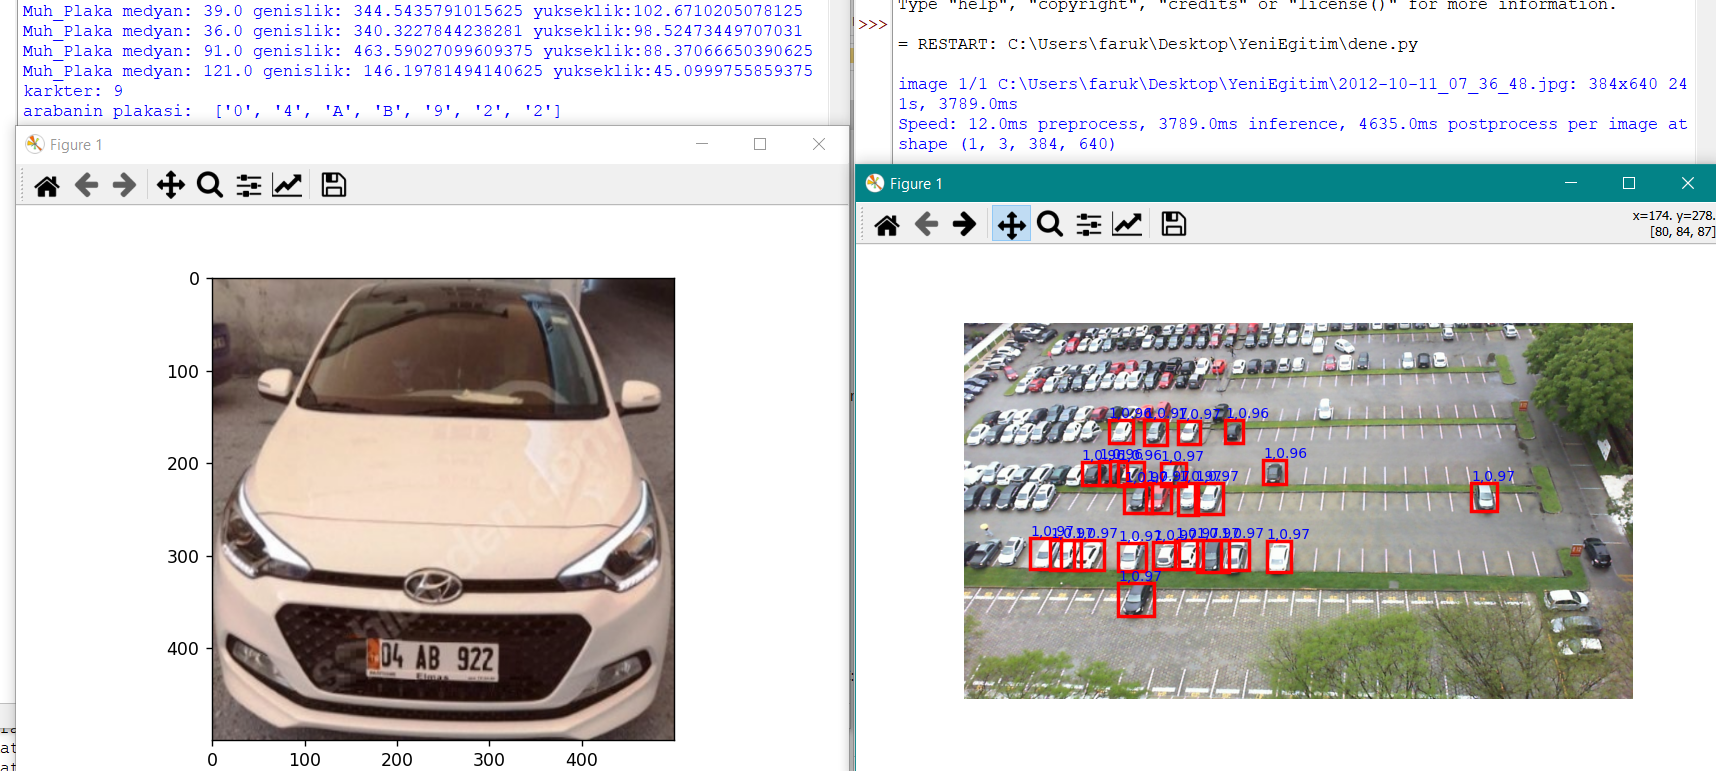
\includegraphics[
		width=13cm,
		height=10cm,
		keepaspectratio,
		]{baslik.png}
		\caption{Eğitim Verilerinin Tablo Çıktıları.}
	\end{figure}
	Bu çalışma, otoparklarda plaka tanıma sistemlerinin geliştirilmesine odaklanmaktadır. Otoparklarda plaka tanıma sistemleri, araçların giriş ve çıkışlarını otomatik olarak yönetmeyi sağlayan önemli bir teknolojidir. Geleneksel yöntemlerin aksine, derin öğrenme tekniklerinin kullanımıyla bu sistemlerin daha doğru ve güvenilir olması hedeflenmektedir. Bu çalışmanın motivasyonu, otoparklarda plaka tanıma sistemleri ile otomatik giriş ve daha sonrasında en yakın otopark alanına yönlendirme üzerine mevcut zorlukları çözmek ve bu sistemlerin performansını arttırmaktır. Üstünde çalışılan proje bittiğinde otopark işletmecilerine ve kullanıcılara önemli avantajlar sağlayacaktır. Örneğin hızlı giriş/çıkış işlemleri, araçların sorunsuz park etme işlemleri, kamera ile güvenlik takibi gibi bir çok özelliği ile birlikte avantaj sağlamaktadır. Bu çalışmanın başlangıç noktası, otopark alanlarında aşırı zaman harcama ve otoparklarda yer bulamama gibi durumlardan kurtulmak adına bazı sınırlamaları belirlemek ve bu sınırlamaları aşmak için yeni bir yaklaşım geliştirmektir. Araştırılan önceki çalışmalarda genellikle az veri seti ile ya da sersör verileri ile sistem çalışmaktadır fakat bu çalışma, bir otopark içerisinde farklı hava koşulları olsa bile kullanılabilecek veri seti ile çalışılmıştır. Bu sayede belli hava koşullarında bile otopark alanı takibi yapabilecektir. Bu çalışmanın önemli parçaları ise otomatik plaka tanıma ve kapı açılışı, doluluk durumunu yapay sinir ağı kullarak eğitilen sistem ile belirleme, kullanılan veri seti ve performans değerlendirme yöntemleri çalışmayı önemli hale gitirmiştir. Bu parçalar, çalışmanın temel bileşenlerini oluşturarak sonuçların güvenilirliğini sağlamıştır. Bu çalışma ile birlikte derin öğrenme tekniklerinin otopark sistemlerinde nasıl geliştirebileceğini göstermektedir.
	
	\section{LİTERATÜR ARAŞTIRMASI}

	Akıllı ulaşım sistemleri ve akıllı şehir uygulamaları, modern şehirlerin karşılaştığı trafik ve park sorunlarına yenilikçi çözümler sunmaktadır. Bu teknolojiler, plaka tanıma ve kamera ile otopark doluluk sistemleri gibi bileşenleri içerir ve otoparkların etkin yönetimi ile sürücülerin en yakın boş park alanlarına yönlendirilmesine olanak tanır. Bu literatür araştırması, plaka tanıma teknolojileri ve kamera tabanlı otopark doluluk sistemlerinin geliştirilmesi ve uygulanması üzerine yapılan çalışmaların, araştırılmış özeti sunulmaktadır.\newline
	
	Plaka tanıma sistemleri (PTS), araç plakalarını otomatik olarak okuyarak tanımlayan ve görüntü işleme teknikleri ile yapay zeka algoritmaları kullanarak çalışan sistemlerdir. PTS'nin yaygın kullanım alanları arasında trafik yönetimi, hız denetimi, otopark yönetimi ve güvenlik uygulamaları bulunmaktadır\cite{makale}. Plaka tanıma sistemleri genellikle üç ana bileşenden oluşur: görüntü alımı, görüntü işleme ve veri analizi ile saklama. Görüntü alımı, kameralar aracılığıyla araç plakalarının görüntülerinin alınmasını içerir. Görüntü işleme, alınan görüntülerin optik karakter tanıma (OCR) teknikleri kullanılarak işlenmesini kapsar. Veri analizi ve saklama aşaması ise tanınan plaka bilgilerinin veri tabanlarına kaydedilmesi ve analiz edilmesini içerir\cite{yavuz}.
	
	Otomatik Plaka Tanıma (OPT) sistemleri, trafik yönetimi ve güvenlik uygulamalarında yaygın olarak kullanılmaktadır. Bu sistemler, araç plakalarının algılanması ve tanınması için genellikle görüntü işleme tekniklerini kullanır. Geleneksel yöntemler genellikle yüksek önişleme gerektirirken, derin öğrenme tabanlı yaklaşımlar, özellikle Maskeli Bölgesel Evrişimsel Sinir Ağları (M-BESA), daha yüksek doğruluk oranları ve daha az önişleme gereksinimi ile öne çıkar. Geleneksel OPT yöntemleri, genellikle plaka yerleştirme, karakter segmentasyonu ve karakter tanıma adımlarını içerir. Bu teknikler, iyi aydınlatılmış ve net görüntülerde başarılı olsalar da değişen ışık koşulları ve kirli plakalar gibi zorlu durumlarda performans düşüklüğü yaşarlar. Derin öğrenme, özellikle son yıllarda OPT alanında önemli ilerlemeler kaydetmiştir. Convolutional Neural Networks (CNN) gibi derin öğrenme mimarileri, görüntüden doğrudan özellik çıkarımı yaparak daha yüksek doğruluk oranları sunar. M-BESA, plaka tanımada karakter maskeleri kullanarak doğruluğu artırır ve karmaşık önişleme adımlarını azaltır. Geleneksel OCR (Optical Character Recognition) yöntemleri, plaka üzerindeki karakterlerin tanınması için kullanılır. Ancak bu yöntemler, karmaşık arka planlar ve çeşitli plaka formatları karşısında zorlanabilir. Derin öğrenme tabanlı OCR yöntemleri, bu tür zorlukları aşmada daha başarılıdır. Literatürde, derin öğrenme tabanlı OPT sistemlerinin geleneksel yöntemlere göre daha yüksek doğruluk ve hız sunduğu belirtilmektedir. M-BESA gibi yaklaşımlar, plaka tanımada doğruluğu artırmakla kalmaz, aynı zamanda sistemin genel verimliliğini de yükseltir\cite{article_515830}.
	
	Otopark doluluk sistemleri, otoparklarda mevcut araç sayısını ve boş park yerlerini belirlemek için kullanılan teknolojilerdir. Bu sistemler, çeşitli kamera türleri ve görüntü işleme algoritmaları kullanarak çalışır. Otopark doluluk sistemleri, dahili ve harici olmak üzere iki ana kategoriye ayrılabilir. Dahili sistemler, araç tespit ekipmanlarının yol yüzeyine monte edilmesiyle uygulanır. İndüksiyon sarmalı sensörler, magnetometreler, manyetik dirençli sensörler gibi çeşitli algılayıcılar kullanılır. Harici sistemler ise araç tespit ekipmanlarının yol yüzeyine veya tavan gibi dış yüzeylere monte edilmesiyle uygulanır. Kameralar, radarlar ve lazer sensörler gibi teknolojiler kullanılarak araçların varlığı ve doluluk oranları tespit edilir. Dahili sistemler genellikle daha hassas ve güvenilir tespit sağlar, ancak kurulum ve bakım maliyetleri yüksektir. Harici sistemler ise daha geniş alanları kapsayabilir ve kurulumu daha kolaydır, ancak çevresel koşullardan daha fazla etkilenebilirler\cite{article_1098978}.
	
	Akıllı otopark sistemleri, araç plakalarının otomatik olarak tanınması ve otopark doluluk durumunun gerçek zamanlı izlenmesi üzerine yoğunlaşan teknolojik çözümler sunar. Python programlama dili, bu sistemlerin geliştirilmesinde sıkça kullanılan bir araçtır. Projenin ilk aşamasında, akıllı otopark sisteminin giriş bölümü için plaka tespit yapısının oluşturulmasına odaklanılmıştır. Python programlama dili kullanılarak veriler veri setinden çekilmiş ve ekrana yansıtılmıştır. Otopark girişinde plakanın kamerada bulunduğu konumu algılayan algoritma için gerekli bilgiler toplanmıştır. Bu süreçte, resimler gri formata çevrilmiş, gürültü ve medyan bulanıklaştırma işlemleri uygulanmıştır. Kenarları algılamak için Jhon Canny Algoritması kullanılmış, ardından plaka karakterlerini seçmek için ayrıştırma ve eşikleme işlemleri gerçekleştirilmiştir. Bu işlemler için kullanılan bilgisayarla görme alanında kullanılan OpenCV kütüphanesi, görüntü işleme ve nesne tespiti için güçlü bir araçtır. Gri tonlama, median bulanıklığı ve adaptif eşikleme gibi teknikler, görüntülerin daha iyi analiz edilebilmesini sağlar. Morfolojik işlemler ve kontur analizi, nesne tespitinde yaygın olarak kullanılan yöntemlerdir ve bu yöntemler sayesinde tespit edilen nesneler görselleştirilebilir. Jhon Canny Algoritması, kenar tespiti için etkili bir yöntemdir ve plaka karakterlerinin ayrıştırılması ve 	eşiklenmesi süreçlerinde önemli bir rol oynar\cite{github}.
	
	Yapay sinir ağlarının temel yapısı, insan beyninin sinir hücrelerinden ilham alınarak tasarlanmıştır. Sinir hücreleri arasındaki bağlantılar, öğrenme süreci boyunca ağırlıklandırılarak bilgi işlemeye ve sonuç üretmeye olanak tanır. Bu ağlar, katmanlı bir yapıdadır ve her katman, belirli bir bilgi işlemeyi gerçekleştirir. Derin öğrenme ise, bu yapının çok katmanlı hale getirilmesiyle ortaya çıkar ve daha karmaşık veri yapılarını ve ilişkileri öğrenme kapasitesine sahiptir. Derin öğrenme de kullanılan YOLO (You Only Look Once) gibi gerçek zamanlı nesne tespit algoritmaları, görüntü ve video analizinde büyük bir devrim yaratmıştır. YOLO algoritması, tek bir sinir ağı ileri besleme ile bir görüntüdeki nesneleri tanımlar ve bunların konumlarını belirler. YOLO'nun en son sürümlerinden olan YOLOv8, daha hızlı ve daha doğru nesne tespiti sağlayarak bu alandaki uygulamalarda yaygın olarak kullanılmaktadır\cite{kitap}\cite{kitap2}.
	
	Yapay sinir ağlarının eğitim süreçlerinde, büyük veri kümelerinin kullanılması gerekmektedir. Bu veri kümeleri, ağın öğrenmesi ve genelleme yapabilmesi için çeşitli örnekler sunar. Ancak, büyük veri kümelerinin işlenmesi ve yönetilmesi, önemli bir zorluk teşkil eder. Bu nedenle, veri işleme ve hazırlık süreçlerinde etkin yöntemlerin kullanılması önemlidir. Özellikle Kaggle gibi platformlar, araştırmacılara ve geliştiricilere çeşitli veri kümeleri sağlayarak bu süreçleri kolaylaştırmaktadır\cite{chatgpt35}.

 	
	\section{YÖNTEMLER}
	Bu rapor, akıllı otopark sistemlerinde plaka tanıma ve araç tespiti üzerine yoğun bir bilgisayarla görme ve yapay zeka çalışmasını kapsamaktadır. Proje, on haftalık bir süreç boyunca kademeli bir yaklaşımı benimsemiştir.
	
	\subsection{Plaka Tespiti ve Tanıma}
	Projenin ilk aşamasında, akıllı otopark sisteminin giriş bölümü için plaka tespit yapısının oluşturulması gerçekleştirilmiştir. Python programlama dili kullanılarak veri setinden çekilen verilerin işlenmesi sağlanmış ve plaka görüntülerinin ekrana yansıtılması gerçekleştirilmiştir. Ardından, otopark girişinde plakanın kamerada bulunduğu konumun algılanması için gerekli bilgiler toplanmıştır. Bu bilgiler arasında dikdörtgen tespiti, plaka boyutları ve boyut oranları gibi özellikler bulunmaktadır. Gürültüyü azaltmak ve plaka karakterlerini belirlemeyi kolaylaştırmak için, görüntüler gri tona dönüştürülmüş ve medyan bulanıklaştırma işlemi uygulanmıştır. Daha sonra, Jhon Canny Algoritması kullanılarak kenarlar algılanmış ve plaka karakterlerinin belirlenmesi için ayrıştırma ve eşikleme işlemleri gerçekleştirilmiştir. Son olarak ise plaka çerçevesi işaretlenerek diğer adıma geçilmiştir\cite{github}.
	
	\begin{figure}[htbp]
		\centering
		\begin{minipage}{0.45\textwidth}
			\centering
			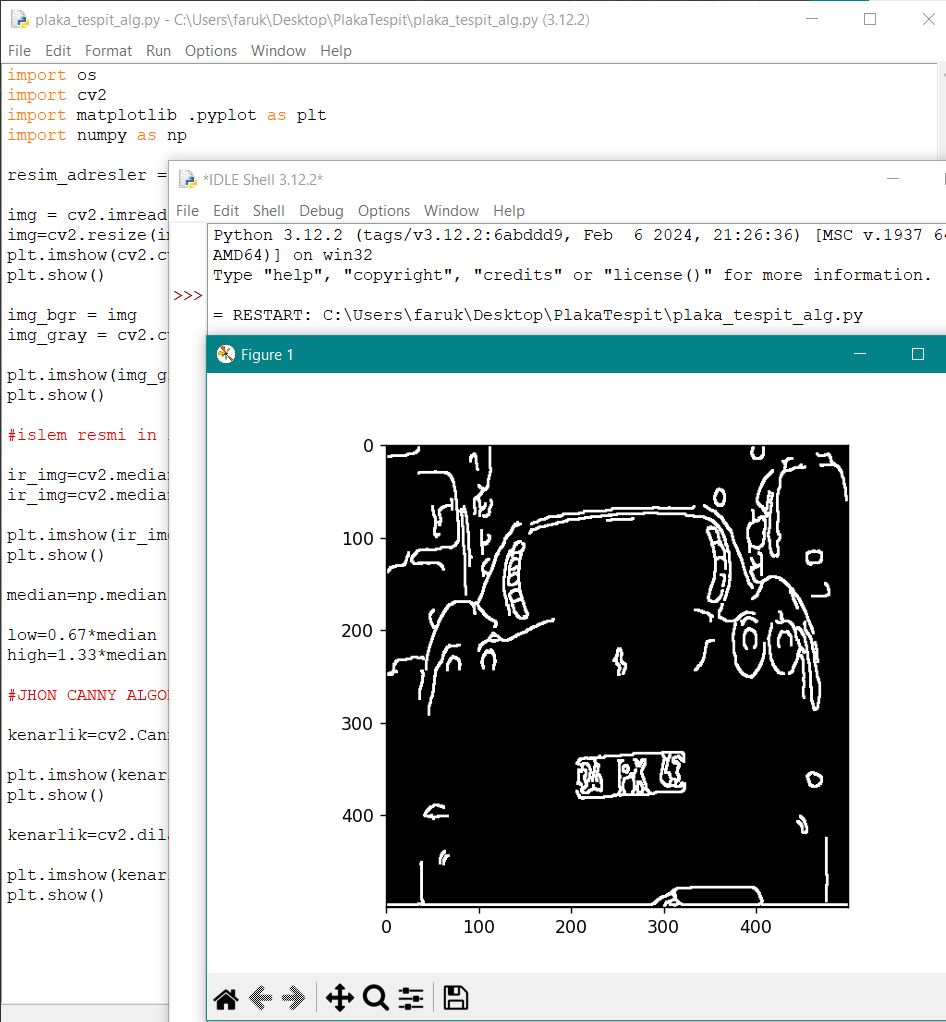
\includegraphics[	
			width=8cm,
			height=7cm,
			keepaspectratio,]{GenisletilmeYapıldı.png}
			\\
			(a)
		\end{minipage}
		\hfill
		\begin{minipage}{0.45\textwidth}
			\centering
			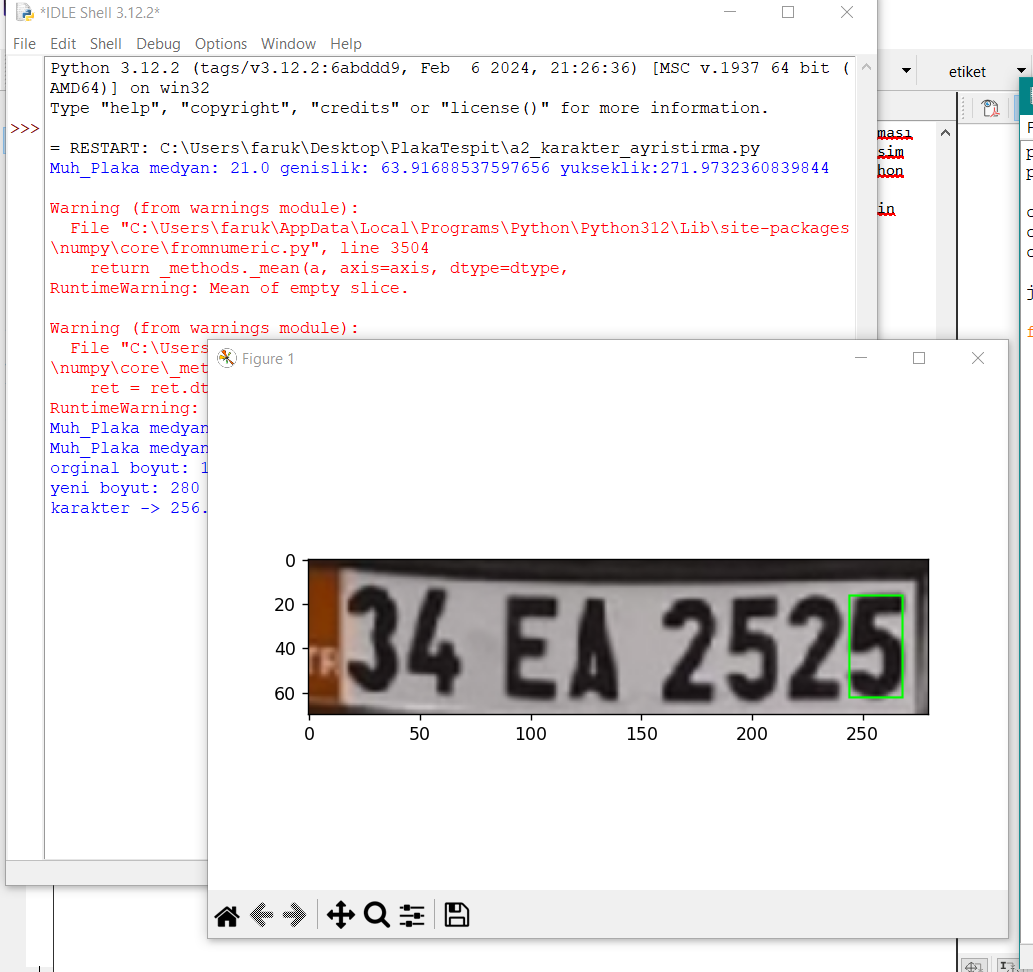
\includegraphics[	
			width=8cm,
			height=7cm,
			keepaspectratio,]{opencv.png}
			\\
			(b)
		\end{minipage}
		\newline
	\end{figure}
	\begin{figure}[!ht]
		\centering
		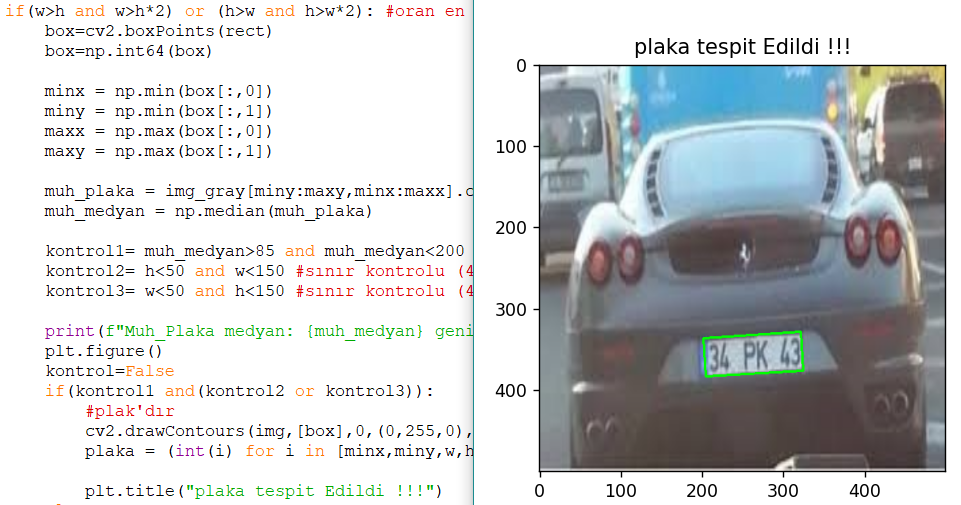
\includegraphics[
		width=10cm,
		height=10cm,
		keepaspectratio,
		]{plakaTespit.png}\\(c)
		\caption{
			{a) Görselin, canny algoritması ve eşiklemeden sonraki hali.}
			{b) Görselde gereken işlemler yapıldıktan sonra plakanın alınması.}
			{c) Görseldeki plakanın tespit edilmesi.}}
	\end{figure}
	\newpage
	\subsection{Makine Öğrenimi Tabanlı Plaka Tanıma}
	 Plaka tanıma sisteminin ikinci aşamasında, plakaları tanımak için RandomForestClassifier makine öğrenimi modeli kullanılmıştır. Bu aşamada, OpenCV ve NumPy kütüphaneleri kullanılarak bir model dosyası (model.joblib) ve sınıf etiketleri belirlenmiştir. Plaka görüntülerinin işlenmesi için gerekli işlevler ve işlem adımları araştırılıp görüntü işleme teknikleriyle plakaların ayıklanması, plaka karakterlerinin tanınması ve tanınan karakterlerin plaka olarak düzenlenmesi gibi işlemler bu aşamada gerçekleştirilmiştir. Bu adımlar, plaka tanıma işlemlerini gerçekleştiren "plakaTani" işlevi içinde yapılmış ve projede kullanılmıştır\cite{github}.
	\begin{figure}[htbp]
		\centering
		\begin{minipage}{0.45\textwidth}
			\centering
			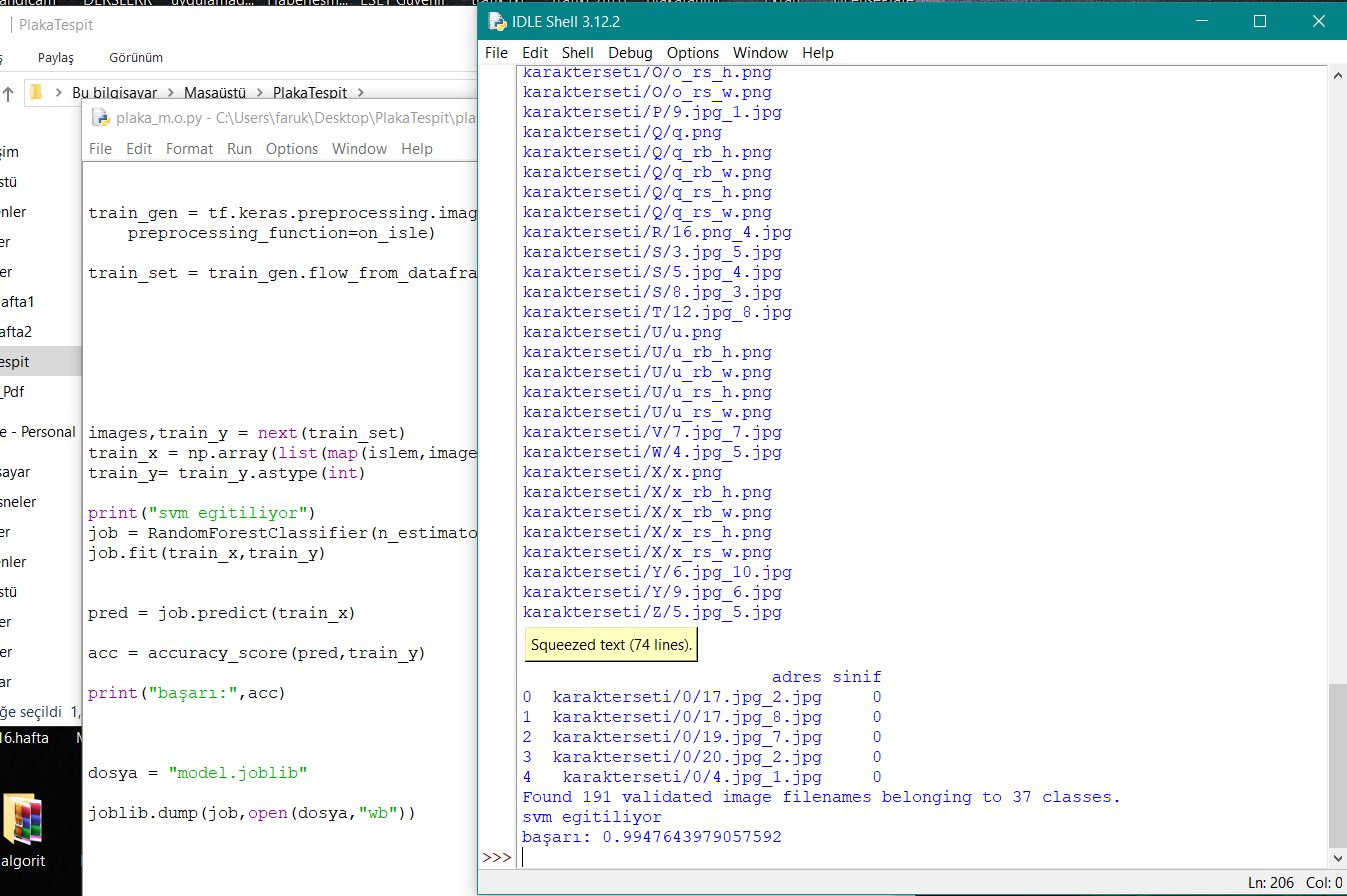
\includegraphics[	
			width=8cm,
			height=7cm,
			keepaspectratio,]{basari.png}
			\\
			(a)
		\end{minipage}
		\hfill
		\begin{minipage}{0.45\textwidth}
			\centering
			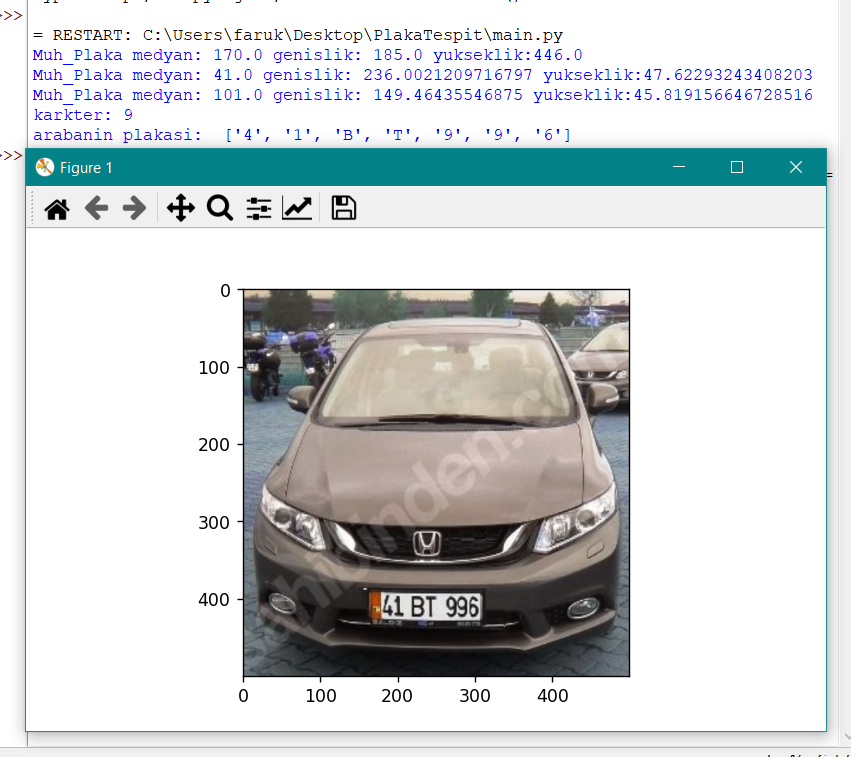
\includegraphics[	
			width=8cm,
			height=7cm,
			keepaspectratio,]{plakaSonuc.png}
			\\
			(b)
		\end{minipage}
		\newline
		\caption{
			{a) Görselin, canny algoritması ve eşiklemeden sonraki hali.}
			{b) Görselde gereken işlemler yapıldıktan sonra plakanın alınması.}}
		
	\end{figure}
		\newpage
	\subsection{Nesne Tespiti ve Takibi}
	Projenin bir diğer odak noktası, bir video dosyasındaki araçların tespit edilmesi ve takip edilmesidir. OpenCV kütüphanesi kullanılarak görüntü işleme teknikleri uygulanmıştır; gri tonlamalı görüntüler elde etmek için renk dönüşümleri, median bulanıklığı ve adaptif eşikleme gibi yöntemler kullanılmıştır. Ardından, morfolojik işlemler ve kontur analiziyle araçlar tespit edilmiş ve bu araçların etrafına dikdörtgenler çizilerek görselleştirilmiştir. Ayrıca, kullanıcı etkileşimli bir arayüz üzerinden nesne tespiti için referans noktalarının belirlenmesini sağlayan bir sistem geliştirilmiştir. Kullanıcı tarafından belirlenen referans noktalarını saklamak için veri yapıları kullanılmıştır ve bu veriler hem pickle formatında hem de CSV dosyalarında saklanmıştır\cite{github}.
	
	\subsection{Otopark Doluluk Durumu Bulma}
	Projenin ikinci aşamasında, başlangıçta Spyder kullanılarak işe başlandı. XML dosyasından veri çekme işlemleri için veriCekme() ve dikdortgenYapma() fonksiyonları tanımlandı. Ardından, OpenCV ve Matplotlib kullanılarak veri işleme adımları gerçekleştirildi. Veri seti, görüntülerin işlenebilmesi için ayrı bir yere alındı. Ayrı yere alınan görüntüler ile hazır araç bulma kodu kullanarak otoparktaki araçların bulunması sağlanmaya çalışıldı\cite{basarasizkod}. Fakat oluşturulan hazır eğitimin dataset görüntüleri projedeki görüntülere uymadığından hazır eğitim otoparktaki araçları bulamadı.
	\begin{figure}[!ht]
		\centering
		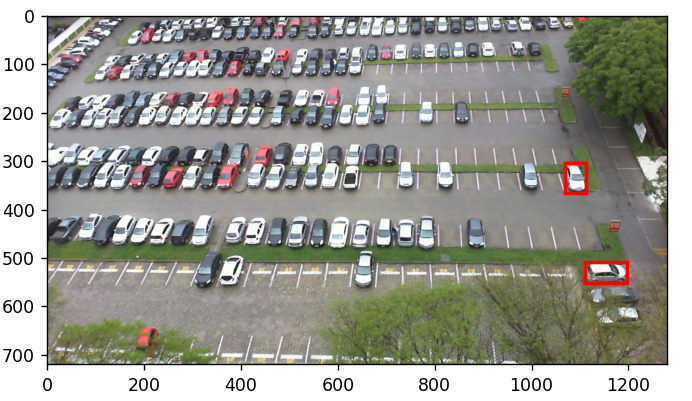
\includegraphics[
		width=12cm,
		height=10cm,
		keepaspectratio,
		]{hazirEgitim.png}
		\caption{Hazır eğitimin projede çalıştırılması.}
	\end{figure}
	
	\subsection{Veri Hazırlama ve Yapay Zeka Eğitimi}
	Projede;hazır eğitimin, projemizde uygun olmamasından dolayı yapay sinir ağı ile yeni eğitim yapılması kararlaştırıldı. Bunun için ilk olarak kullanılacak olan yapay zeka modeli için veri bulma ve veriyi hazırlama aşamasına geçildi. Bu adımlarda, öncelikle Kaggle gibi platformlardan uygun veri setleri bulunmuş ve gerekli veriler çekilerek işlenmiştir\cite{dataset}. Ardından, verilerin etiketlenmesi ve veri setinin oluşturulması için gerekli bilgiler toplanmıştır. Veri setleri, dolu otopark alanlarını içerecek şekilde ayrılmış ve eğitim için uygun hale getirilmiştir. Veri işleme adımlarında roboflow sitesi kullanılarak veri işleme aşaması tamamlanmıştır\cite{roboflow}. Son olarak, eğitim ve test verileri ilgili klasörlere kopyalanmış ve yapay zeka modelinin eğitimine hazır hale getirilmiştir.
	
	\begin{figure}[!ht]
		\centering
		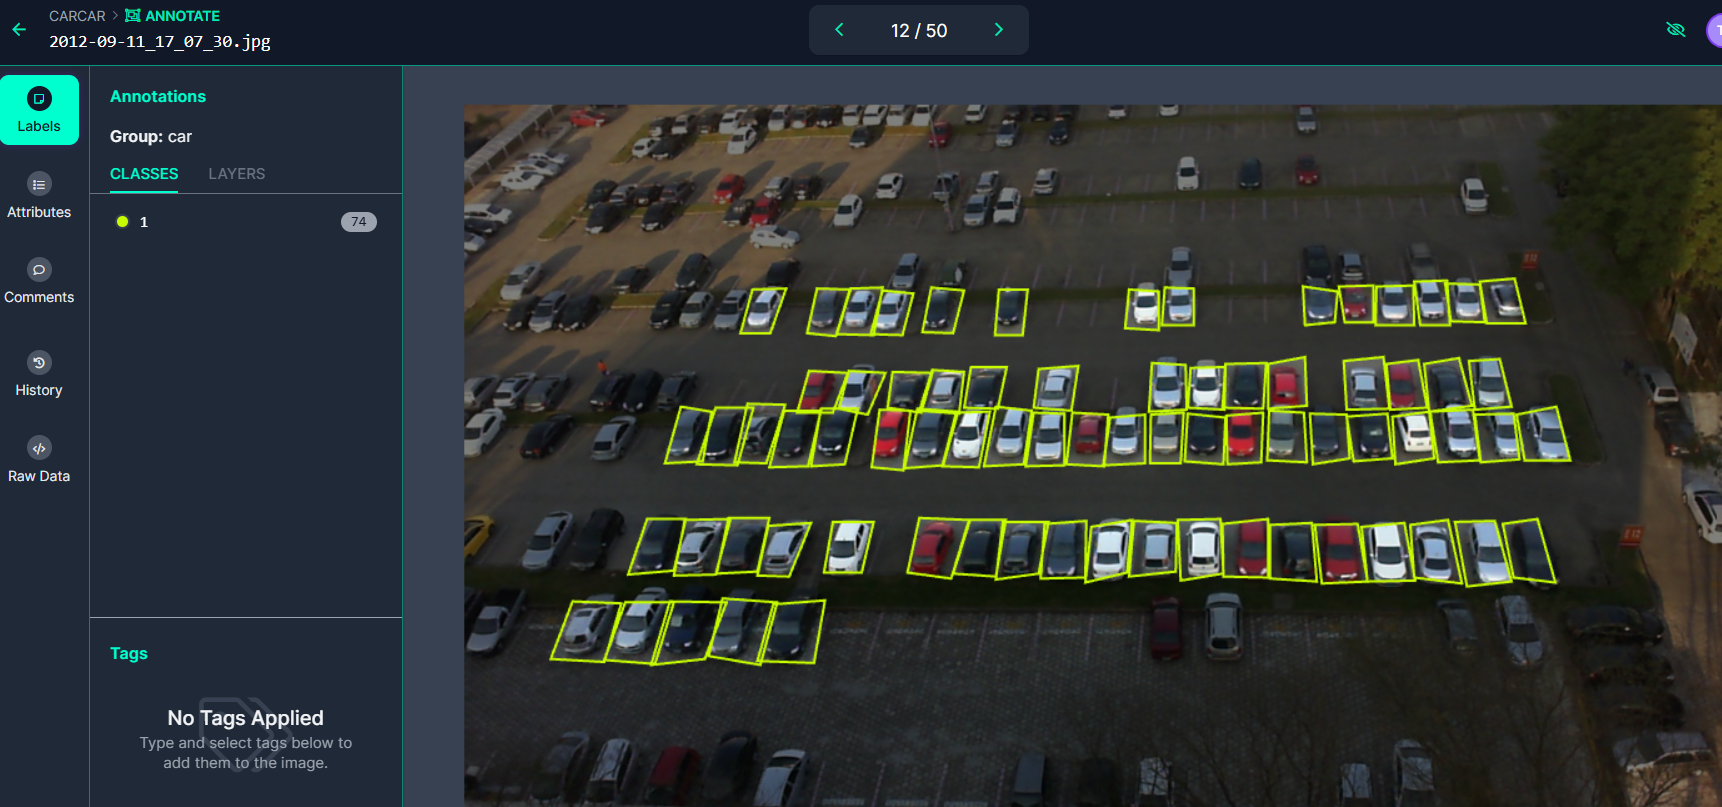
\includegraphics[
		width=12cm,
		height=10cm,
		keepaspectratio,
		]{dataset1.png}
		\caption{Yapay sinir ağı eğitimi için dataset hazırlanması.}
	\end{figure}
	\newpage
	\subsection{Yapay Sinir Ağları ve Model Optimizasyonu}
	Projenin son aşamasında, yapay sinir ağlarının derinlemesine incelenmesine ve model optimizasyonuna odaklanılmıştır. Literatür taraması ve internet kaynaklarından elde edilen bilgilerle birlikte, YOLOv8 gibi güncel yapay sinir ağı modelleri üzerine araştırmalar yapılmış ve ilgili kodlar incelenmiştir. Kodların uygulanması sırasında yaşanan sorunlar ve çözüm yolları araştırılmış, örnek eğitimler yapılarak modelin davranışları ve performansı incelenmiştir\cite{kod2}. Daha sonra gerçek eğitime geçilerek eğitime başlanmıştır\cite{yapayZekaKod}. Eğitim sırasında yaşanan sorunlar, uygun çözüm yolları bulunarak aşılmış ve modelin eğitimi başarıyla tamamlanmıştır. Kullanılan yolo modeli sayesinde eğitim bittikten sonra eğitim parametleri otomatik olarak çıkartıldı. Çıkan gerekli parametreler incelenerek eğitimin başarısı değerlendirilip projeye entegre edildi. Yapılan eğitim örnek otopark fotoğraflarında da denendikten sonrada olumlu sonuçlar alınmıştır.
	\begin{figure}[!ht]
		\centering
		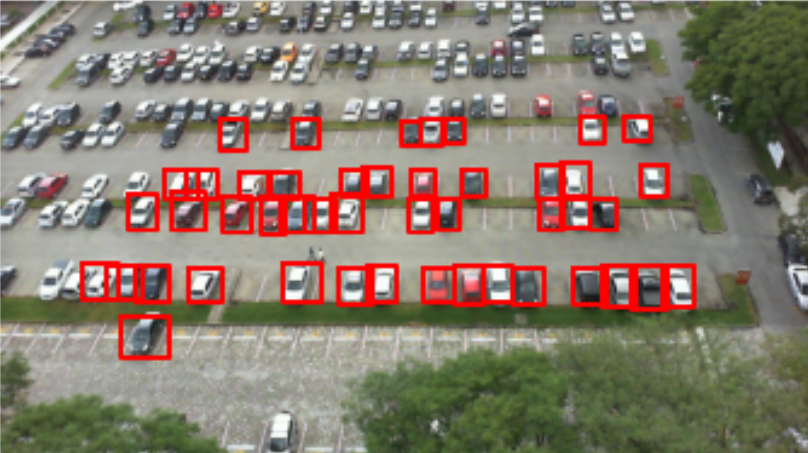
\includegraphics[
		width=12cm,
		height=10cm,
		keepaspectratio,
		]{egitimSonuc.png}
		\caption{Bitirilen eğitimin projede denenmesi.}
	\end{figure}
	\newpage
	\section{BULGU VE TARTIŞMA}
	Bu çalışma, akıllı otopark sistemlerinde plaka tanıma, araç tespiti ve doluluk belirleme üzerine bir dizi yöntem ve teknik incelenmiştir. Her bir adımda farklı yaklaşımlar denendi ve elde edilen bulguların analizi yapıldı.
	\subsection{Otopark Doluluk Sistemi Eğitiminin Sonuçları}
	Bu bölümde, Otopark doluluk sistemi için yapılan yapay sinir ağı eğitimi hakkında bilgi ve değerlendirme sonuçları verilmiştir.
	
	\subsubsection{Confusion Matrix Tablosu}
		\begin{figure}[!ht]
			\centering
			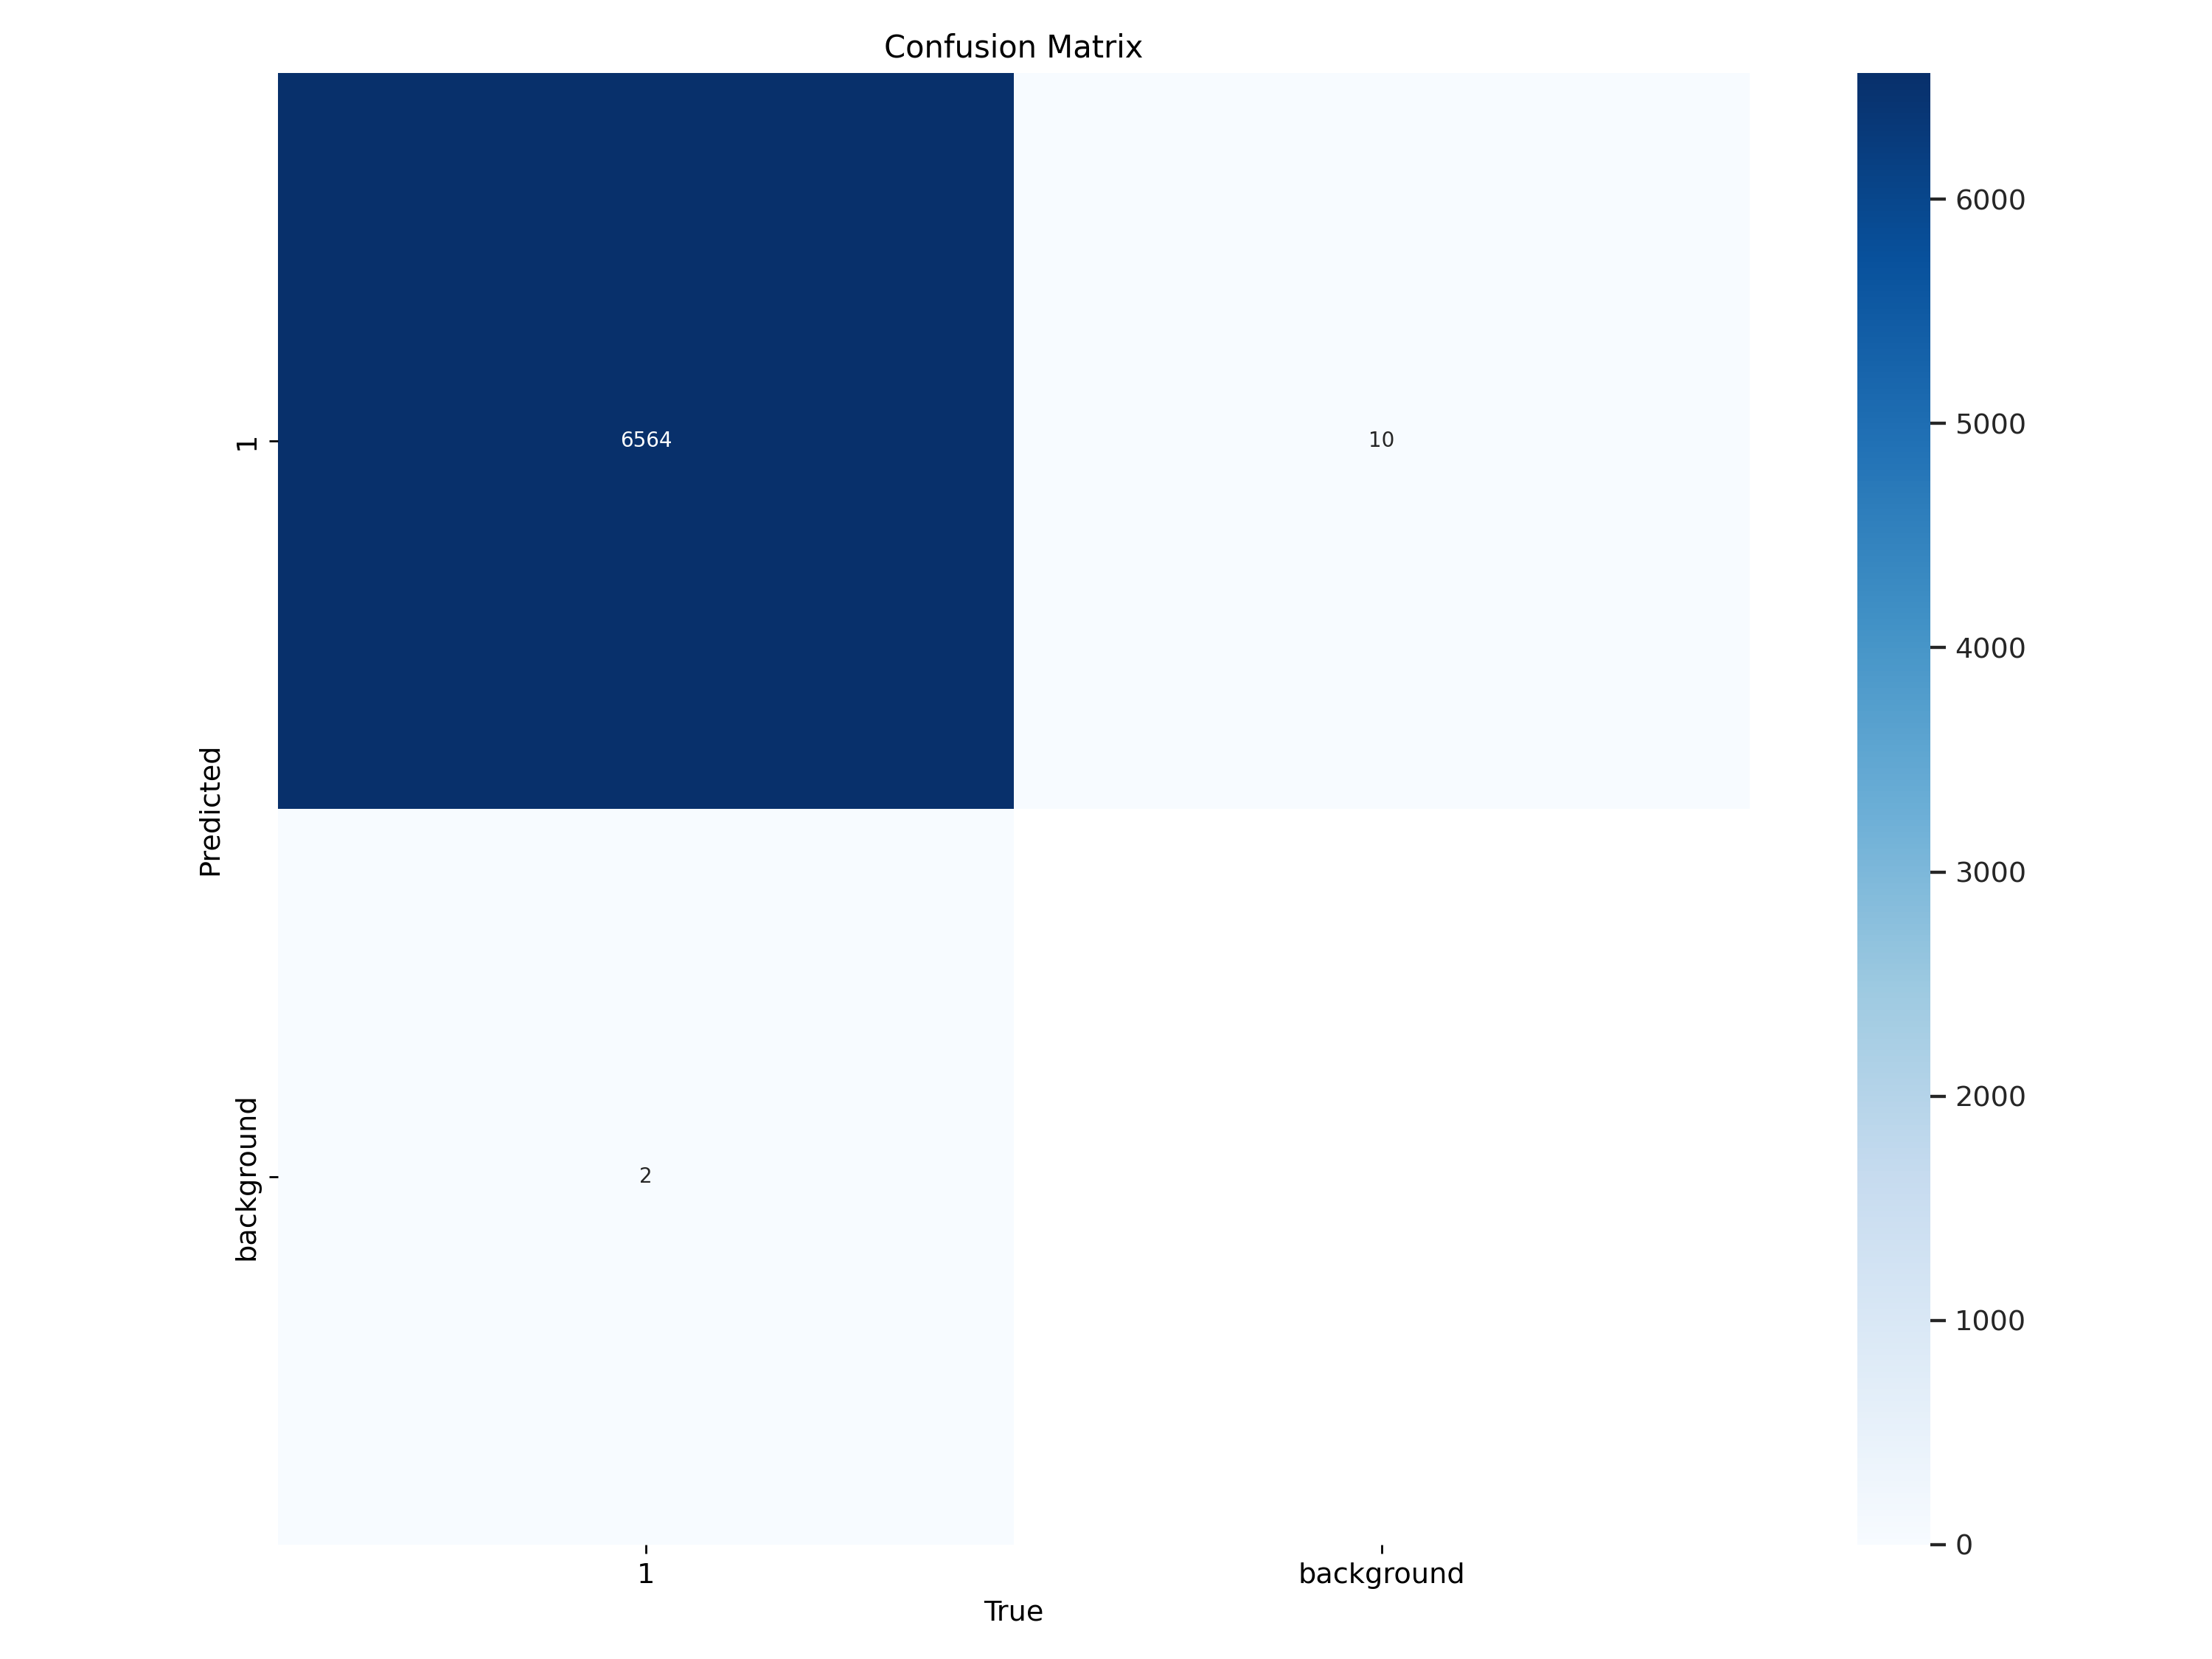
\includegraphics[
			width=10cm,
			height=10cm,
			keepaspectratio,
			]{confusion_matrix.png}
			\caption{Eğitimin Confusion Matrix Çıktısı.}
			
		\end{figure}

		\begin{itemize}
			\item Confusion Matrix (Karmaşıklık Matrisi), bir sınıflandırma modelinin performansını görsel olarak gösteren bir tablodur. Bu tablo, modelin gerçek ve tahmin edilen sınıflarını gösterir ve doğru veya yanlış tahminlerin sayısını belirtir. True Positives (TP), True Negatives (TN), False Positives (FP) ve False Negatives (FN) olmak üzere dört kategori vardır. Karmaşıklık matrisi, modelin ne kadar doğru çalıştığını anlamak için kullanılır ve modelin geliştirilmesine yardımcı olur.
		\end{itemize}
		\newpage
	\subsubsection{Eğitim Çıktı Sonuçlarının Tablosu}
		\begin{figure}[!ht]
			\centering
			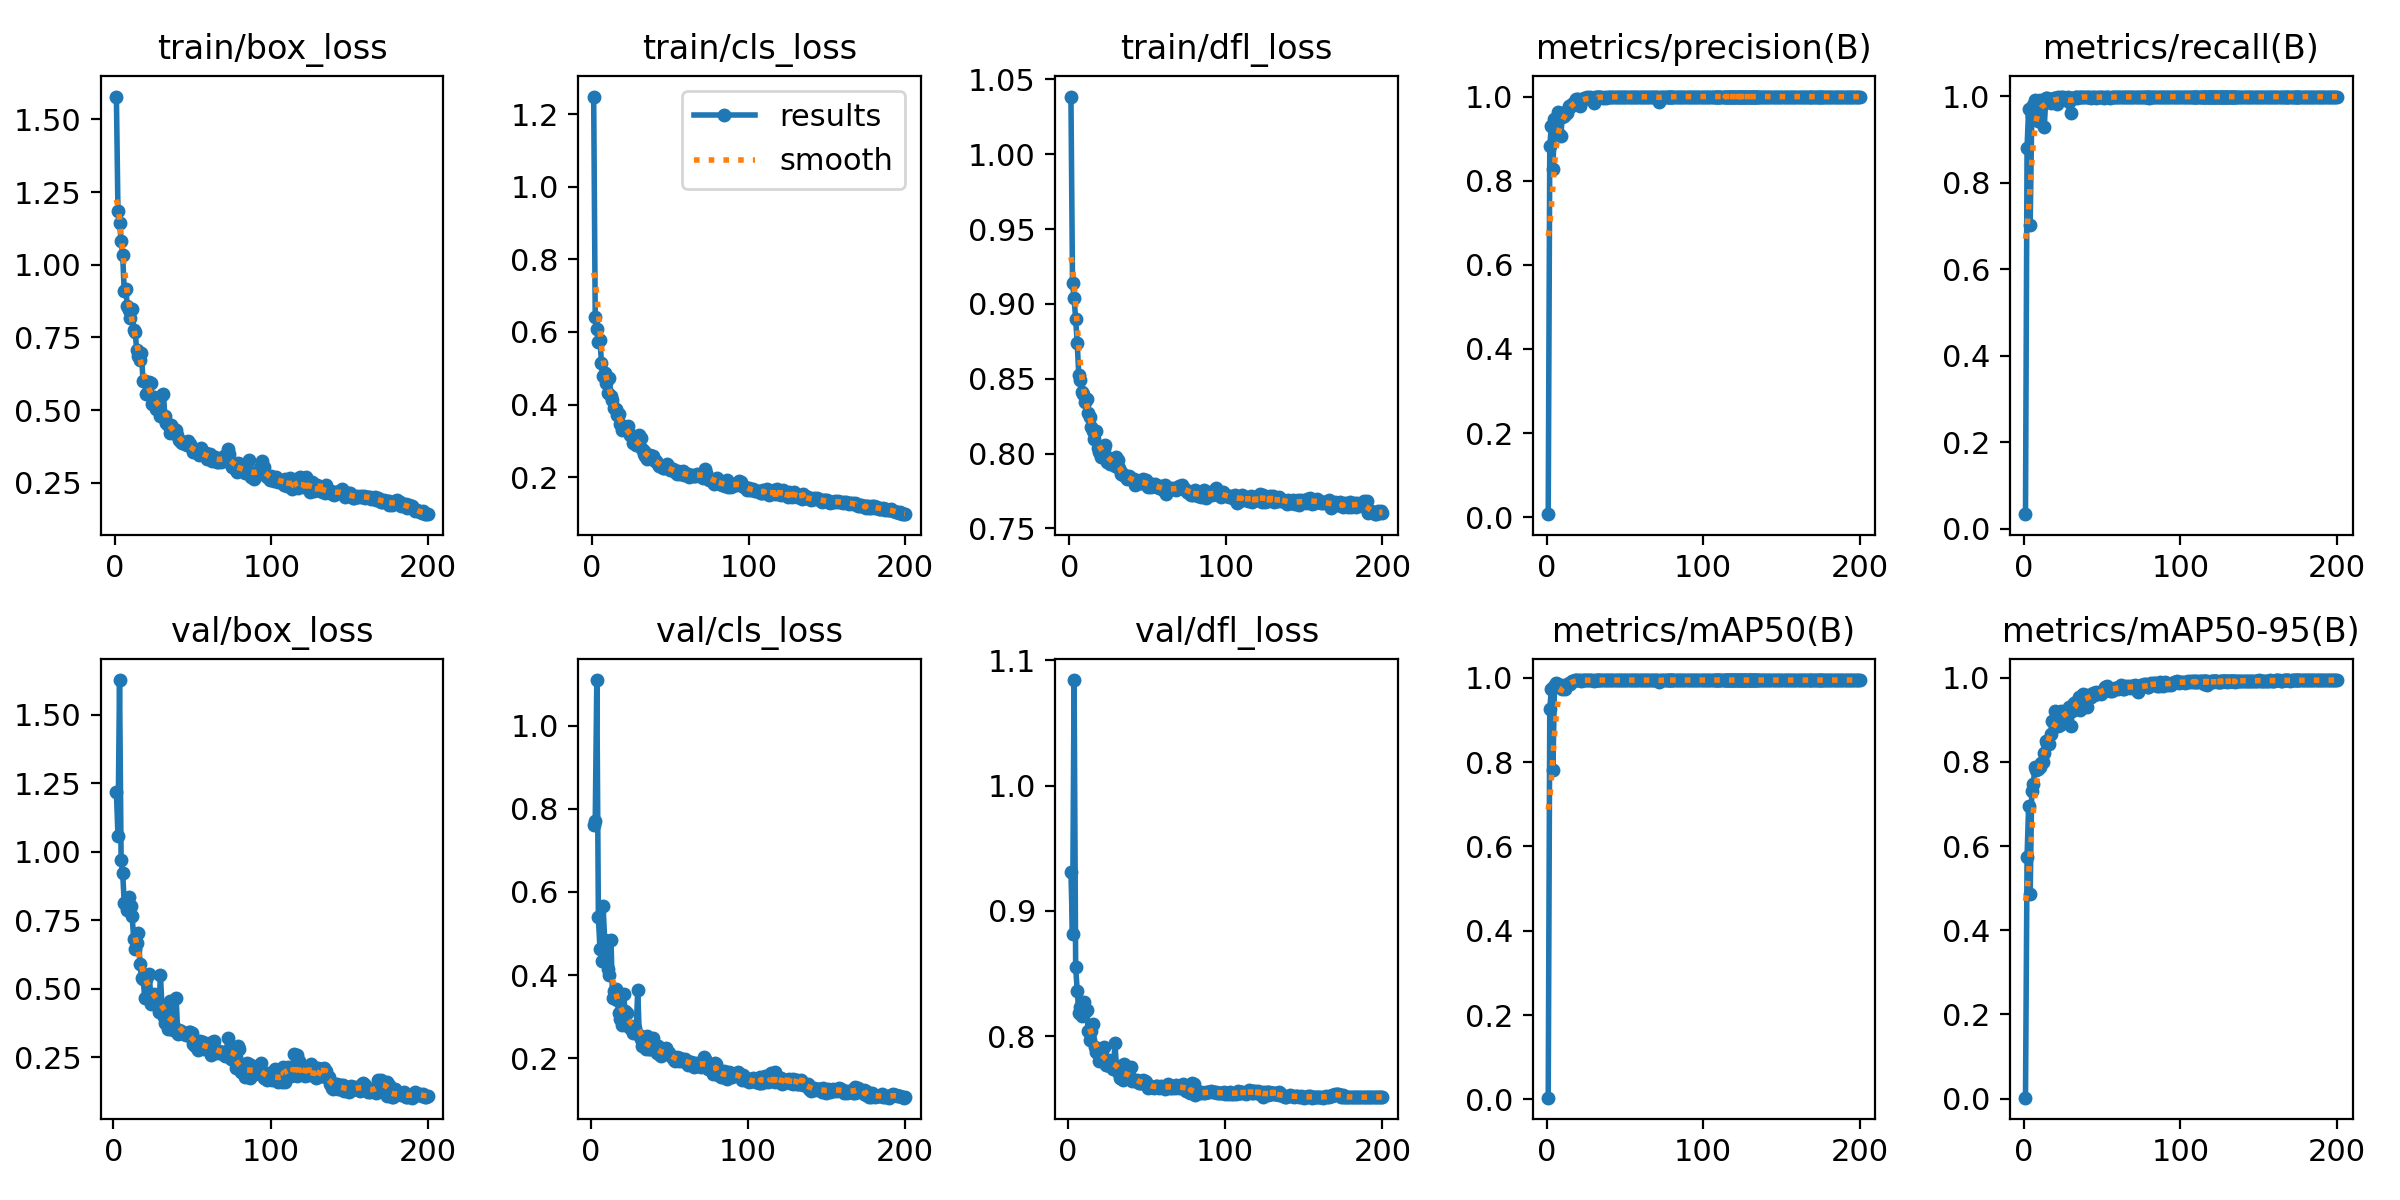
\includegraphics[
			width=15cm,
			height=10cm,
			keepaspectratio,
			]{resultsE.png}
			\caption{Eğitim Verilerinin Tablo Çıktıları.}
		\end{figure}
		\begin{itemize}
			\item Box\_loss, nesne dedektörlerinin eğitimi sırasında kullanılan bir metriktir. Bu metrik, nesne dedektörlerinin tahminlerinin gerçek nesne konumlarıyla ne kadar uyumlu olduğunu ölçer. Yani, model ne kadar doğru nesne konumları tahmin edebiliyorsa, "box\_loss" o kadar düşük olur.
			\item Cls\_loss; nesne dedektörlerinin eğitimi sırasında kullanılan metrik, modelin nesnelerin sınıflarını doğru bir şekilde tahmin edip edemediğini ölçer. Yani, model ne kadar doğru sınıflandırma yapabiliyorsa, "cls\_loss" o kadar düşük olur.
			\item dfl\_loss, dedektörlerin nesne konumlarını daha hassas bir şekilde tahmin etmeye odaklanan özel bir kayıp fonksiyonunu ifade eder. Yani, model ne kadar doğru ve hassas nesne konumları tahmin edebiliyorsa, "dfl\_loss" o kadar düşük olur. Bu tablonun sonucu ise modelin nesneleri daha doğru bir şekilde sınıflandırdı mı ve nesne konumlarını daha iyi belirledi mi bakmamıza yardımcı olur.
			\item Precision(kesinlik), modelin pozitif olarak tahmin ettiği örneklerin ne kadarının gerçekten pozitif olduğunu gösterir.Aşağıda gösterilen denklem \ref{precision},Precision'un formülüdür.
			\begin{equation}
				 \text{Precision} = \frac{\text{True Positives}}{\text{True Positives} + \text{False Positives}}
				 \label{precision}
			\end{equation}
			\item Recall, gerçek pozitif örneklerin doğru bir şekilde saptanma oranını ölçer. Recall'in matematiksel olarak ifade edilmiş hali, doğru pozitiflerin toplam pozitif tahminlere oranıdır. Yani, recall değeri ne kadar yüksekse, modelin gerçek pozitif örnekleri doğru bir şekilde tanımlama yeteneği o kadar iyidir. Örneğin, bir recall değeri 1'e ne kadar yakınsa, modelin tüm gerçek pozitifleri doğru bir şekilde saptadığı anlamına gelir. Aşağıda gösterilen denklem \ref{recall},Recall'in formülünü göstermektedir.
			\begin{equation}
				\text{Recall} = \frac{\text{True Positives}}{\text{True Positives} + \text{False Negatives}}
				\label{recall}
			\end{equation}
		\end{itemize}
	\newpage
	\subsubsection{Validasyon Eğitim Çıktısı}

		\begin{figure}[!ht]
			\centering
			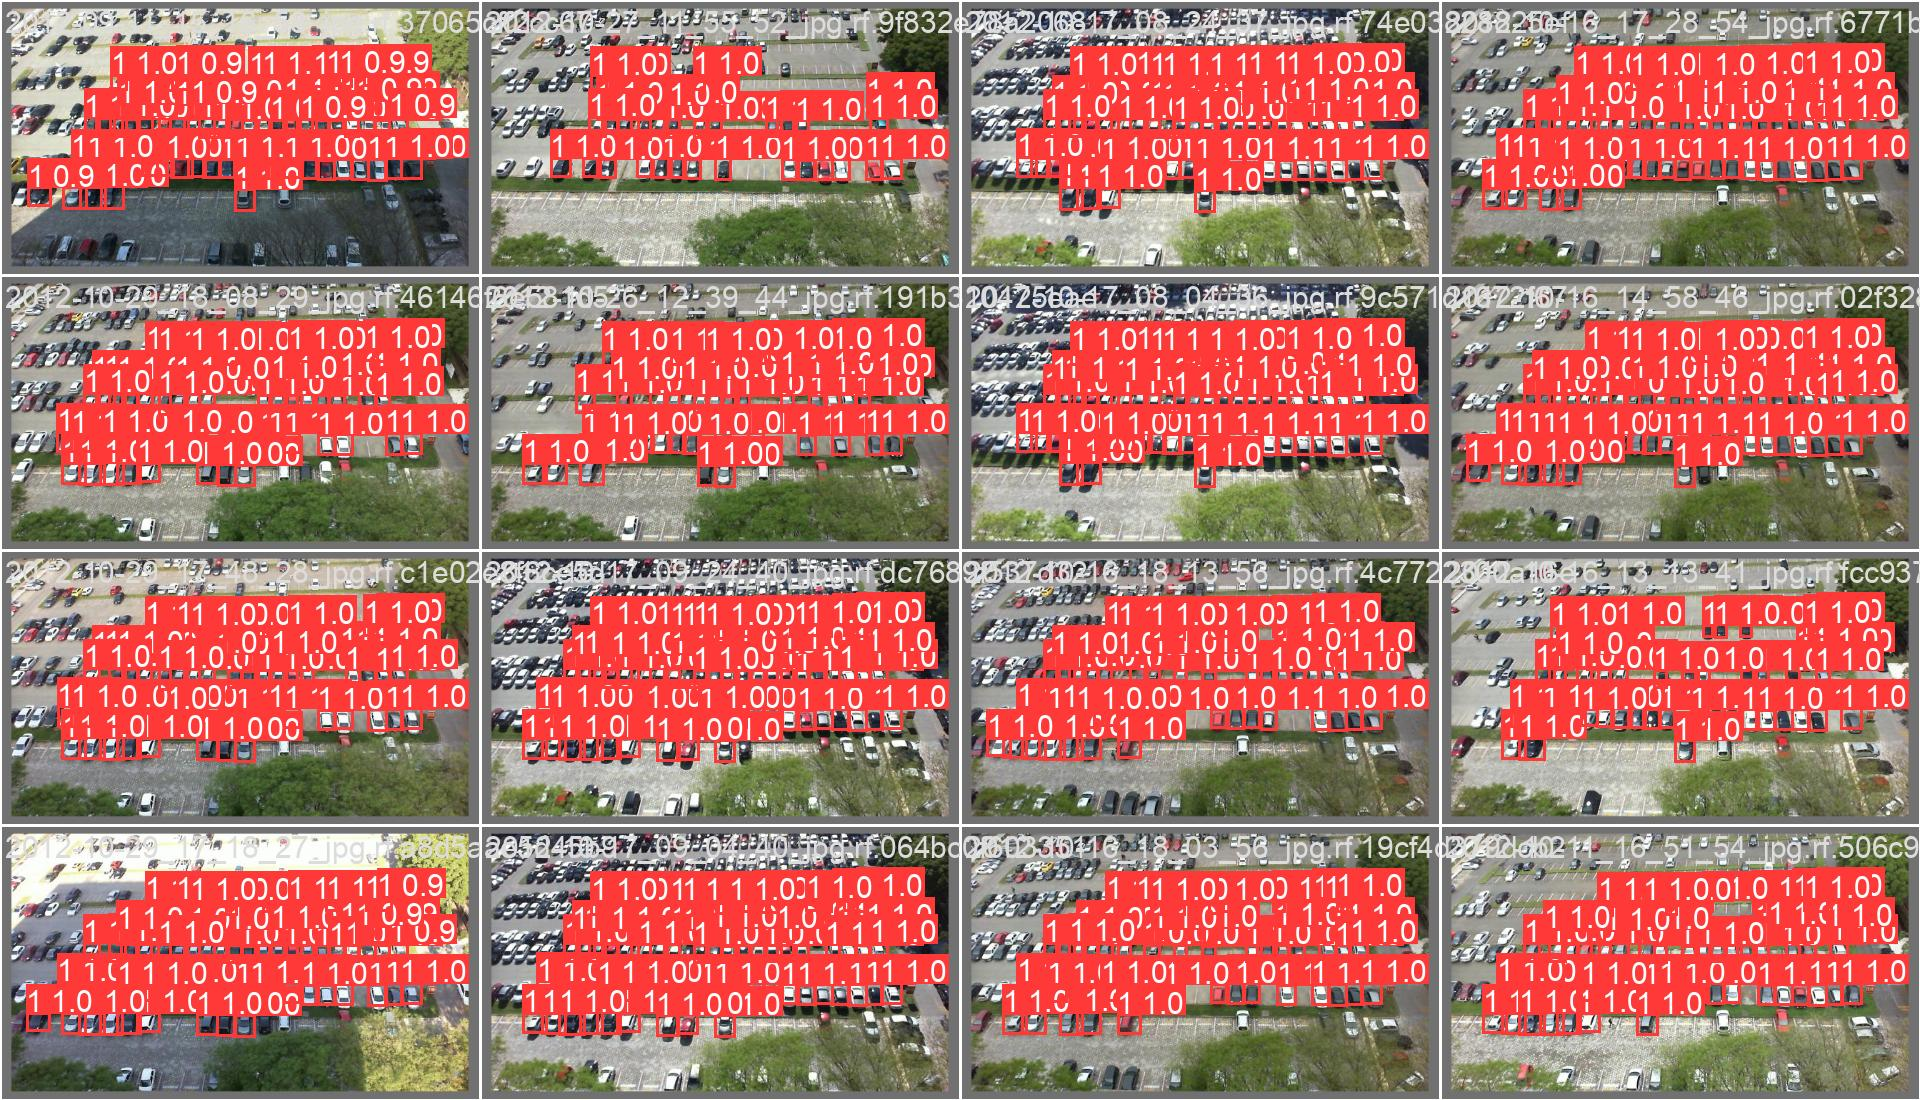
\includegraphics[
			width=12cm,
			height=10cm,
			keepaspectratio,
			]{val_batch0_pred.jpg}
			\caption{Örnek validasyon eğitim çıktısı.}
		\end{figure}
    
	Otopark Doluluk sisteminin yapay sinir ağı ile yapılan ve yolov8 modeli kullanılan eğitimin validasyon çıktısında, araçların bulunduğu görülmektedir. Araçların sık olmasından dolayı bazı yerlerde dikdörtgenlerin taştığı fakat bunun bir sorun yaratmadığı düşünülmektedir.

	\subsection{Veri seti Bilgileri}
	Bu bölüm, projede kullanılan veri setleri hakkında bilgi vermektedir.
	
	\subsubsection{Plaka Tanıma Sistemi Veri seti Bilgileri}
	Plaka tanıma sistemi projesi için kullanılan dataset, github'da bulunan hazır eğitim klasörünün içinden alınmıştır. Datasette, harflerin ve sayıların klasörleri vardır. Bu klasörler içinde de plakarlardan alınmış tagler bulunmaktadır. Her klasörde aşağı yokarı 5-10 tane örnek fotoğraf bulunmaktadır. Eğitimin kalitesini artırmak için ekstra fotoğraflar da eklenmiştir\cite{github}.
	
	\begin{figure}[!ht]
		\centering
		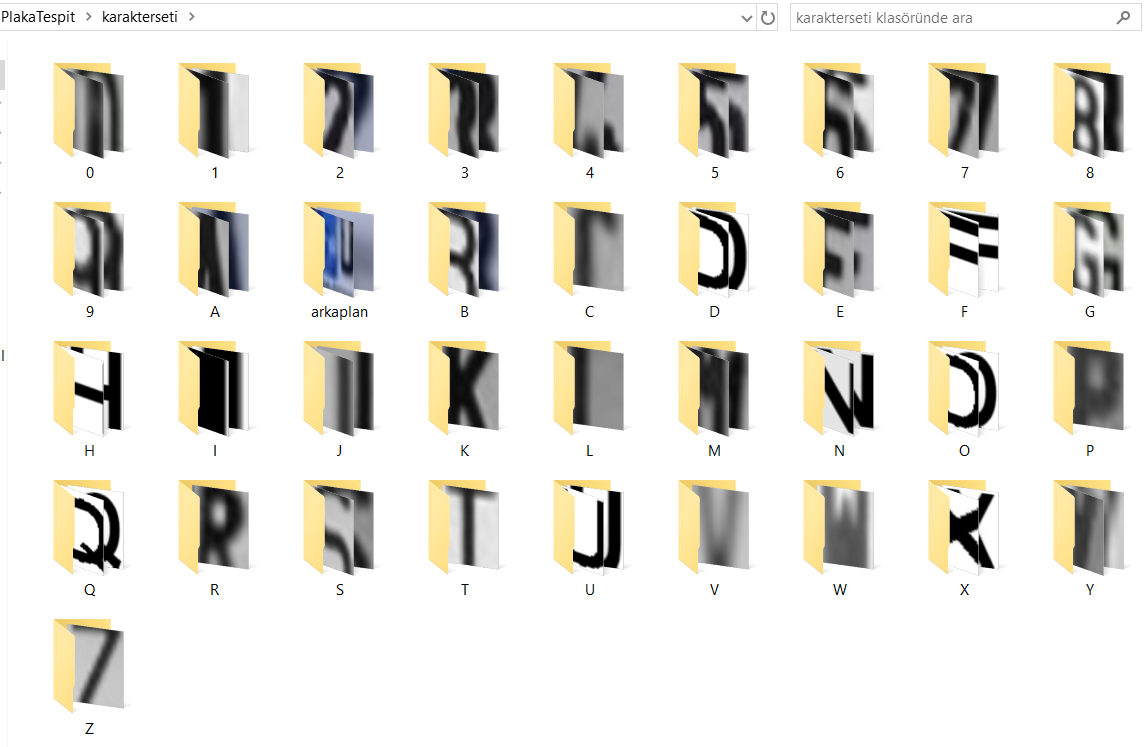
\includegraphics[
		width=10cm,
		height=10cm,
		keepaspectratio,
		]{plakaTespitD.png}
		\caption{Plaka tespit sistemi eğitimi için kullanılan dataset.}
	\end{figure}
	\newpage
	\subsubsection{Otopark Doluluk Bulma Sistemi Veri seti Bilgileri}
	Otopark projemizde kullanmak üzere kaggledan veri seti araştırıldı. Bulunan veri seti, 11gb veri bulundurmaktadır. 3 tane otopark bölgesinin fotoğraflarını; güneşli,bulutlu ve yağmurlu  olmak üzere üstten fotoğrafları çekilmiş olarak sunulmuştur. Her otopark bölgesi için 1000 den fazla fotoğraf bulunmaktadır. Veriler etiketlenerek .xml dosyasına kaydedilmiştir. Ayriyeten etiketlenerek kesilmiş boş ve otopark bölgesinde araçlı olarak fotoğraflar kesilerek toplu fotoğraflar dışında fotoğraf klasörü oluşturulmuştur. Bir tane otopark bölgesi seçilerek o otopark bölgesine ait fotoğraflar alınarak eğitim için hazırlanmıştır. Yapılan eğitimde de 990 tane fotoğraf alınarak eğitimde kullanılmıştır.\cite{dataset}.
	
	\begin{figure}[!ht]
		\centering
		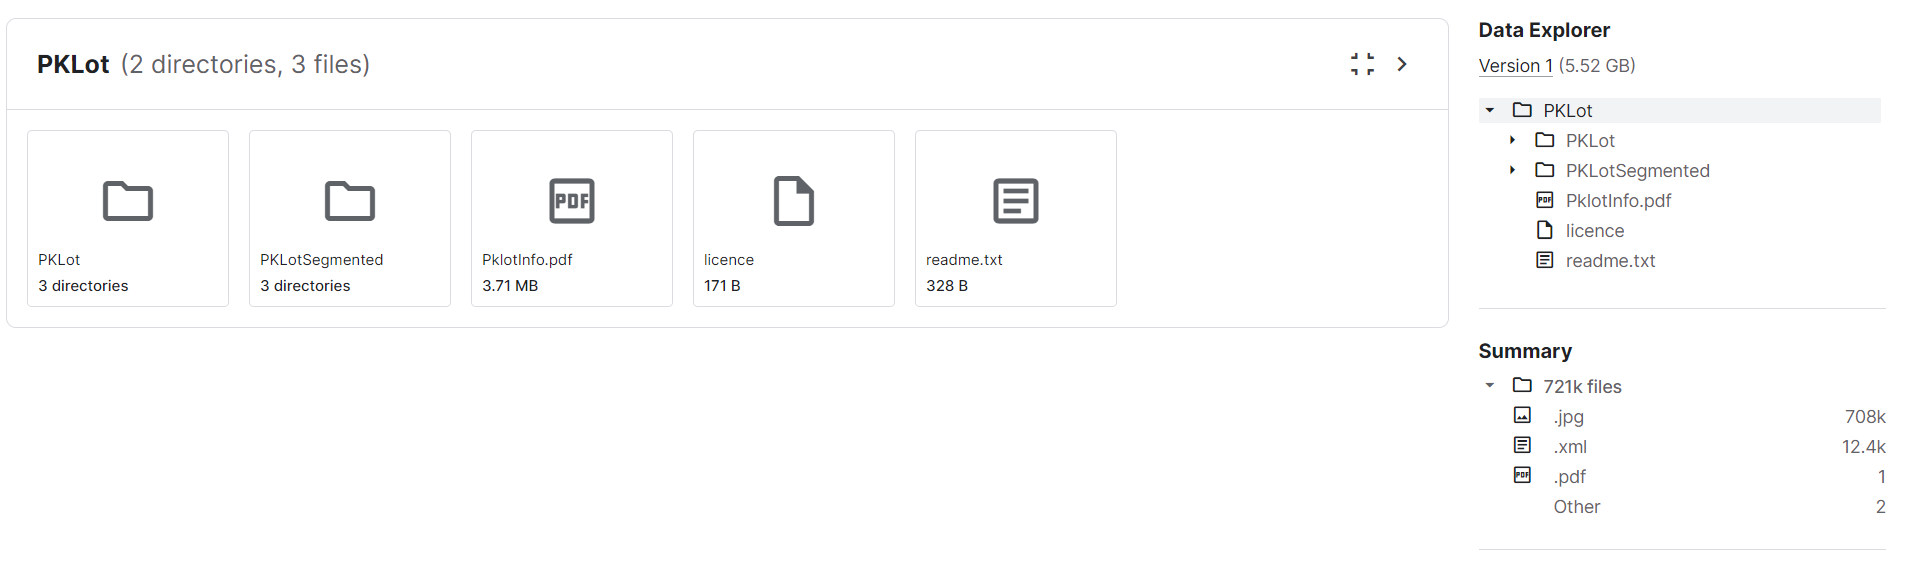
\includegraphics[
		width=13cm,
		height=10cm,
		keepaspectratio,
		]{datasetlis.png}
		\caption{Verilerin işlenerek otopark alanlarının işaretlenmesi}
	\end{figure}
	
	\subsection{Plaka Tespiti ve Tanıma}
	Plaka tespiti ve tanıma adımlarında, görüntü işleme ve makine öğrenimi teknikleri kullanılarak başarılı sonuçlar elde edildi. Görüntülerin işlenmesi için kullanılan algoritmalar, plakaların doğru bir şekilde tespit edilmesini ve karakterlerinin tanınmasını sağladı. Ancak, yapılan eğitimde veri azlığından dolayı tam öğrenim sağlanamadı ve belli bir eşik değeri sayısı kullanıldığı için plakanın bulunamaması ya da yanlış sonuçların çıkması durumlarıyla karşılaşıldı. Bu yüzden de bazı durumlarda plakaların tespit edilmesinde hala zorluklar yaşanması nedeniyle karakter tanıma doğruluğunun iyileştirilmesi gerektiği gözlemlendi.
	\begin{figure}[htbp]
		\centering
		\begin{minipage}{0.43\textwidth}
			\centering
			\includegraphics[	
			width=8cm,
			height=7cm,
			keepaspectratio,]{plakaTanımama.png}
			\\
			(a)
		\end{minipage}
		\hfill
		\begin{minipage}{0.43\textwidth}
			\centering
			\includegraphics[	
			width=8cm,
			height=7cm,
			keepaspectratio,]{plakatanıma.png}
			\\
			(b)
		\end{minipage}
		\newline
		\caption{
			{a) Plaka tanıma algoritmasının hatalı tanıması.}
			{b) Plaka tanıma çıkarımının yapılamaması nedeniyle arabanın plakasının okunamaması.}}
	\end{figure}
	
	\subsection{Otopark Doluluk Sistemi Eğitiminde Roboflow Sorunları}
	Otopark doluluk sistemine yönelik eğitim veri setinin derlenmesi roboflow web sitesi üzerinden yapıldı ancak bazı sorunlarla karşılaşıldı. Öncelikle belirli bir miktardan fazla veri verildiğinde yükleme süresi uzamakta ve yüklenme sorunu oluştuğu düşünülmektedir fakat yavaş yükleme nedeniyle beklenmesi gerekmektedir. Projede verilerin yüklenmesi 40 dakika sürmüştür. İkinci sorun ise Roboflow'ta eğitimleri tamamlayıp proje kodunu aldıktan sonra veri setinin tekrar kullanılmasına izin vermemesi ve eğitim kodunu vermemesidir. Bu nedenle ya kodun başka bir yerden bulunup projeye entegre edilmesi ya da farklı bir veri seti hazırlanması gerekmektedir\cite{roboflowSite}.
	\begin{figure}[!ht]
		\centering
		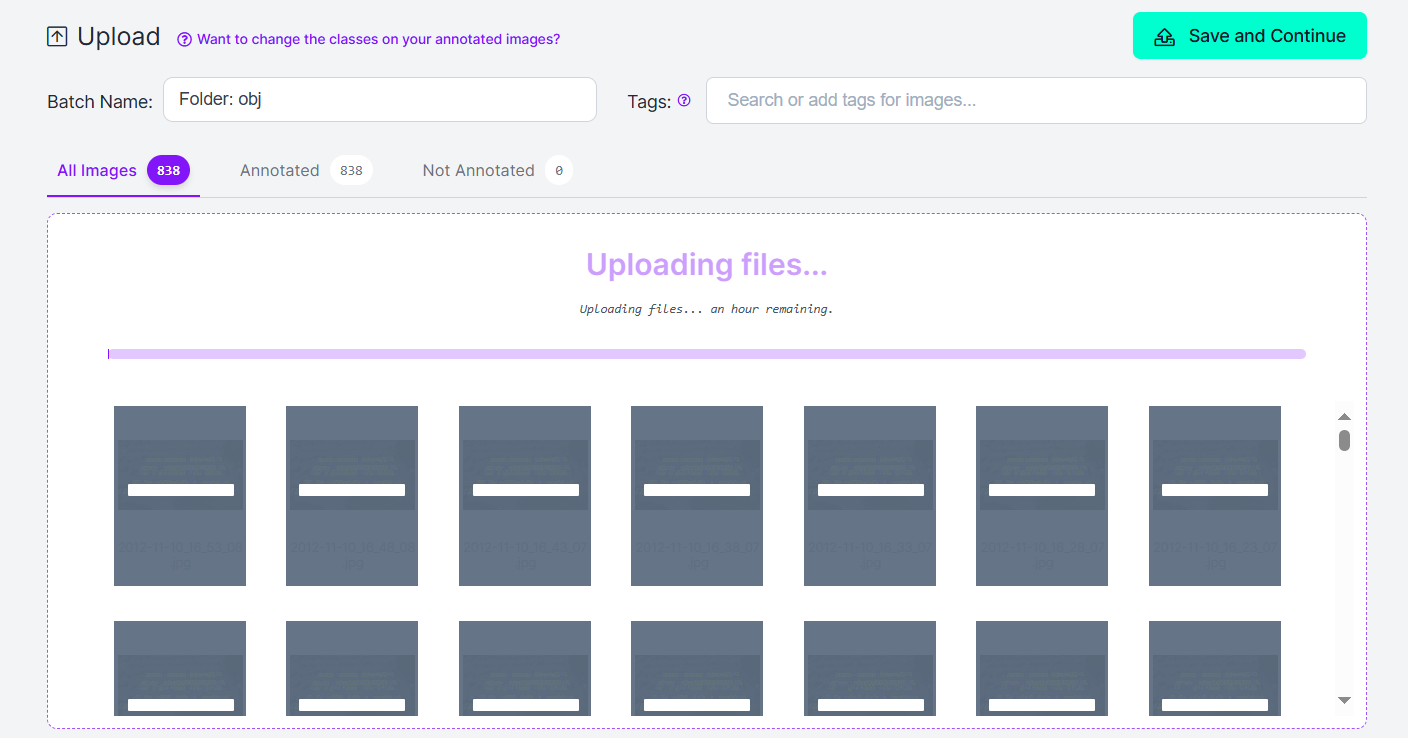
\includegraphics[
		width=10cm,
		height=10cm,
		keepaspectratio,
		]{ornek.png}
		\caption{Roboflow uzun süre aran yüklenme sorunu.}
	\end{figure}
	
	\subsection{Hazır Eğitimin Otopark Doluluk Sistemine Uygun Olmaması}
	Otopark doluluk sisteminde kullanılmak için hazır araç bulma eğitimi kullanılarak projenin süresi kısaltılmaya çalışılmış ve proje daha kısa sürede bitirilmesi istenmiştir. Ayriyeten otoparkta park eden araçlar dışında da diğer araçları takip ederek optimize bir sistem yapmak amaçlanmıştır fakat hazır eğitim ile yapılan değerlendirmeler ve otopark sistemindeki araçların diğer datasete uygun olmamasından dolayı istenilen sonuç elde edilememiştir. Bu yüzden de projeye özgü yeni eğitim yapılmıştır\cite{basarasizkod}.
	
	\begin{figure}[!ht]
		\centering
		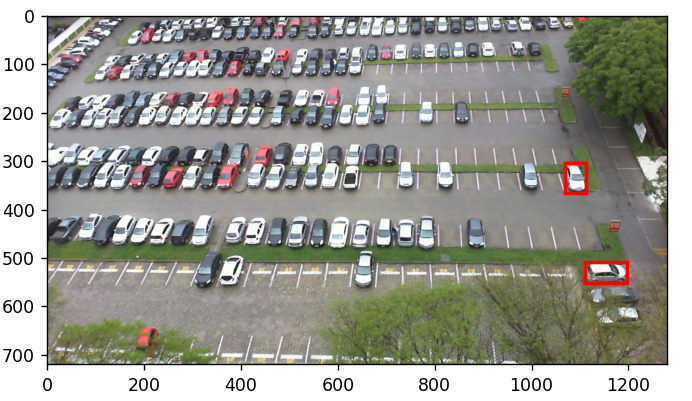
\includegraphics[
		width=12cm,
		height=10cm,
		keepaspectratio,
		]{hazirEgitim.png}
		\caption{Hazır eğitimin projede çalıştırılması.}
	\end{figure}
	
	\subsection{Colab'da Yapılan Eğitimde Çıkan Sorunlar}
	Otopark doluluk sistemi için YOLOv8 modelinin eğitimi için Colab üzerinde bir çalışma gerçekleştirildi. Ancak, Colab'ın sınırlı çalışma süresi nedeniyle eğitim sürekli olarak yarıda kesiliyordu\cite{colab}. Bu sorunu çözmek için eğitim sürecini düzenli aralıklarla kaydedebilmesi gerekiyordu. Bunun için de ek kodlar ultralytic'in web sitesinden alındı ve çalışmaya entegre edildi\cite{kod2}. Ayrıca, eğitimlerin Colab üzerinde kaydedilmesi nedeniyle, süre sona erdiğinde eğitimlerin silinmesi sorunu, Google Drive'a kaydetme seçeneği eklenerek çözüldü. Bu sayede eğitimlerin kaybolması önlenmiş oldu.
	\begin{figure}[htbp]
		\centering
		\begin{minipage}{0.43\textwidth}
			\centering
			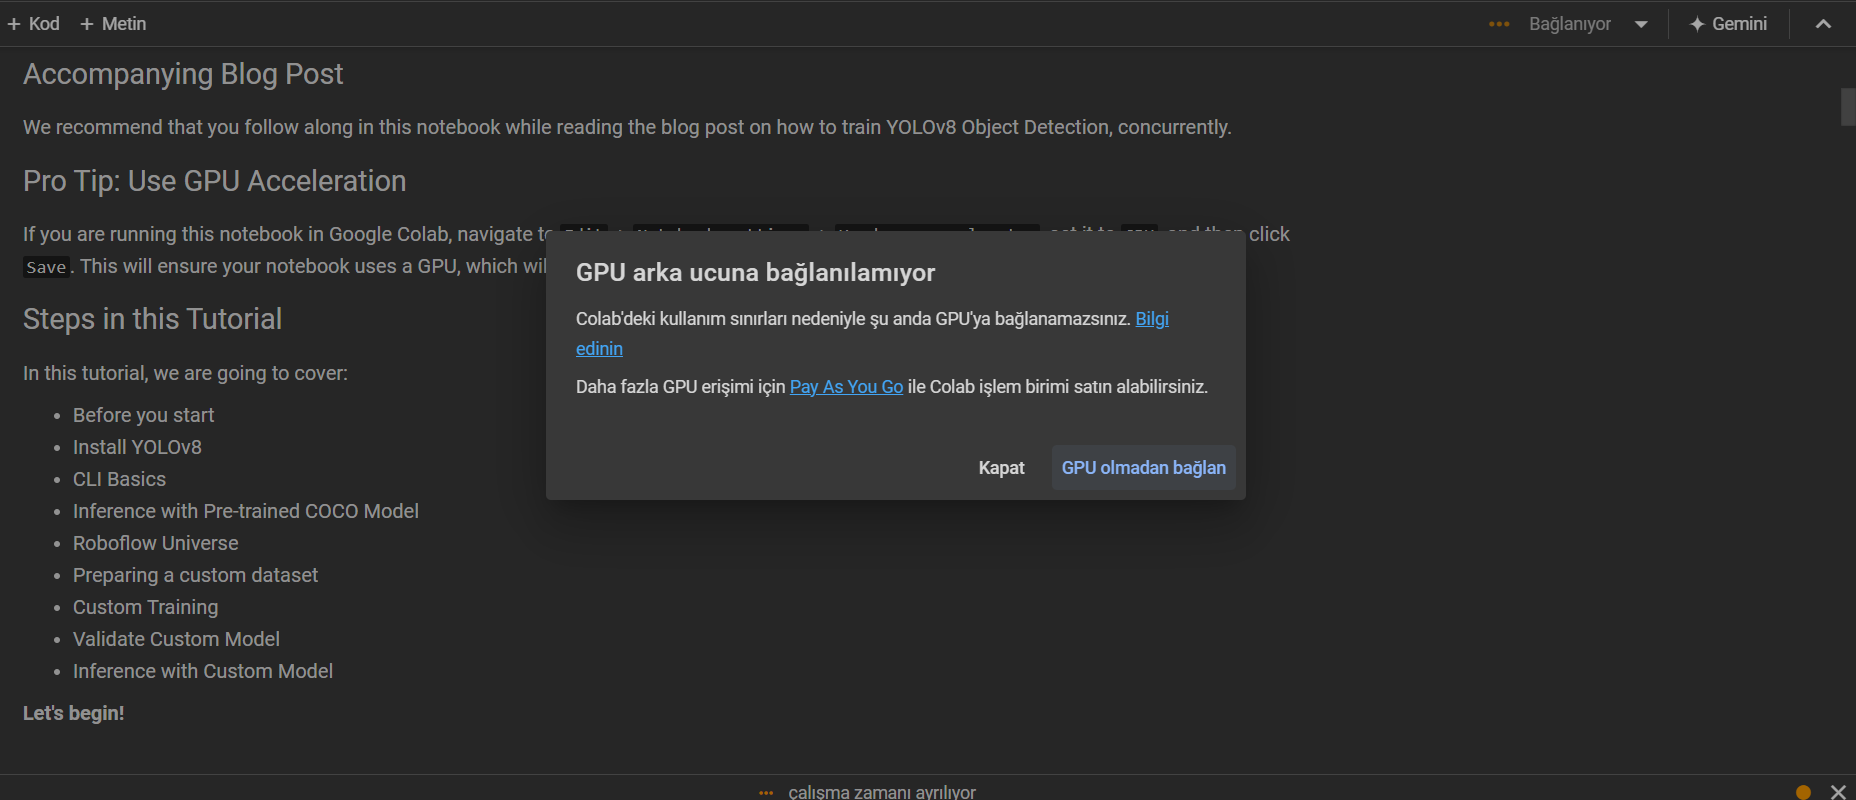
\includegraphics[	
			width=8cm,
			height=7cm,
			keepaspectratio,]{gpuHata.png}
			\\
			(a)
		\end{minipage}
		\hfill
		\begin{minipage}{0.43\textwidth}
			\centering
			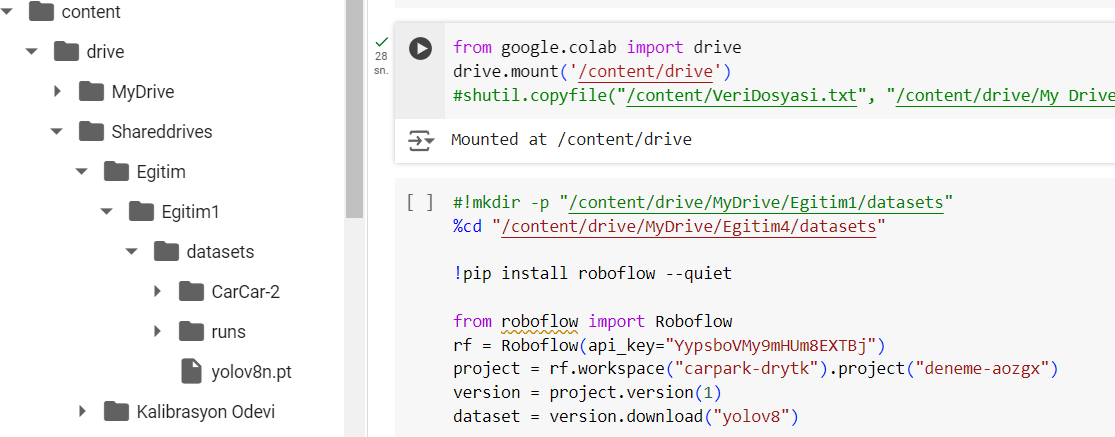
\includegraphics[	
			width=8cm,
			height=7cm,
			keepaspectratio,]{kaydetme.png}
			\\
			(b)
		\end{minipage}
	\end{figure}
	\begin{figure}[!ht]
		\centering
		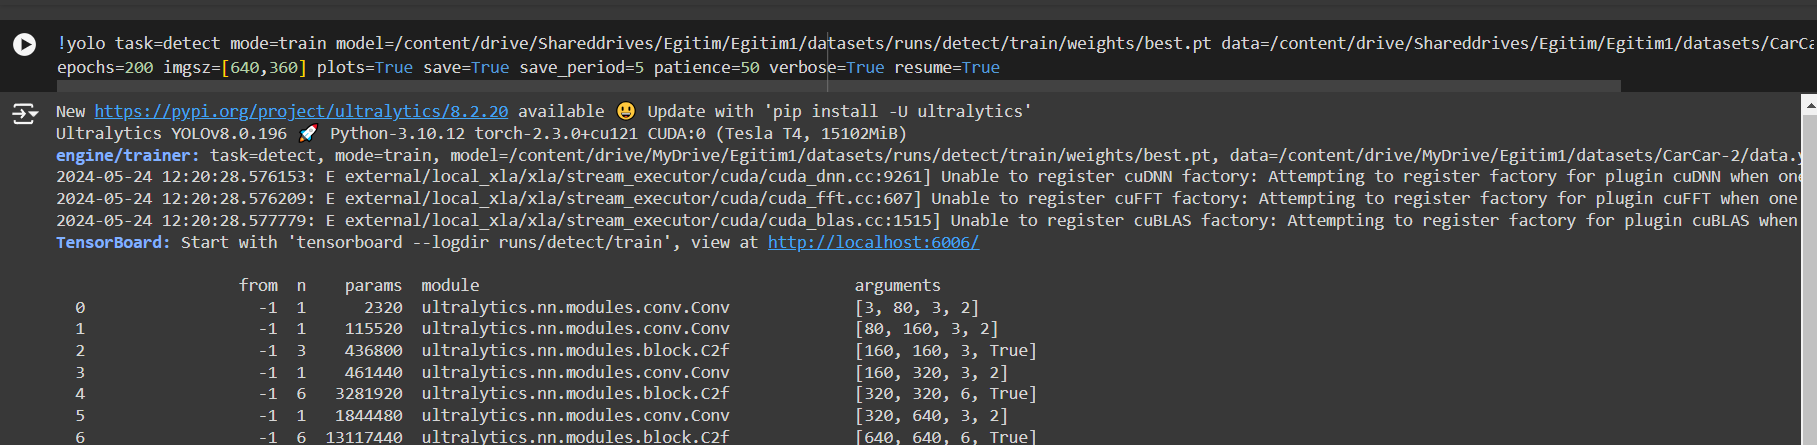
\includegraphics[
		width=15cm,
		height=10cm,
		keepaspectratio,
		]{kod1.png}
		\\	(c)
		\caption{
			{a) Colab süresinin dolmasından dolayı eğitimin aksaması.}
			{b) Colabda dosyaların drive'a kaydedilerek eğitimin devam etmesi.}
			{c) Yolov8 eğitimin kaldığı yerden devam etmesi için düzenlenmiş kod.}}
	\end{figure}
	
	\subsection{Yolov8 Eğitiminin Sürekli Yenilenmesi Durumu Sorunu}
	Otopark doluluk sistemi için yapılan eğitim sürecinde, sürekli eğitimin yeniden başlaması nedeniyle yeni kodların test edilmesi için küçük bir veri seti oluşturuldu ve bu veri seti üzerinde kodların işleyişinin doğrulanması amaçlandı. Ancak, eğitim süreci boyunca result.png dosyasının oluşturulması için aralıklı olarak eğitim durdurulduğunda, bu dosyanın eğitim tamamlandıktan sonra oluşturulduğu gözlendi. Result.png dosyasının eğitim sırasında da oluşturulabilmesi için gerekli kod arayışları sürdürüldü. Bu arayışlar sonucunda, ultralytic'in web sitesinde bulunan kod kullanılarak result.png dosyası eğitim tamamlanmadan da üretilebildi\cite{result}. Daha sonra, eğitim sürecinin baştan mı başladığı yoksa kaldığı yerden mi devam ettiği, kaydedilen loss ve hassasiyet değerlerine bakılarak belirlendi. Bu değerlerin incelenmesiyle, eğitim sürecinin kesintiye uğramadan devam ettiği ve modelin belirli bir noktadan itibaren gelişim kaydettiği görüldü.
	
	\begin{figure}[htbp]
		\centering
		\begin{minipage}{0.43\textwidth}
			\centering
			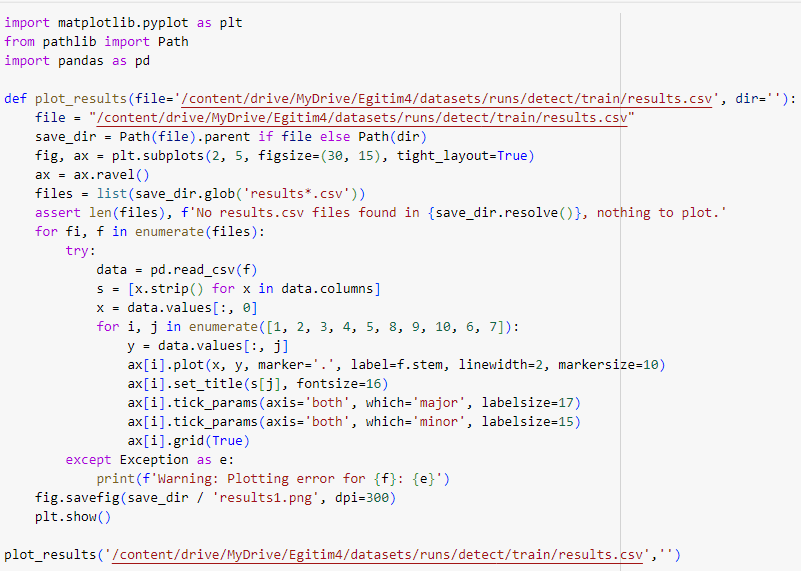
\includegraphics[	
			width=8cm,
			height=7cm,
			keepaspectratio,]{kod2.png}
			\\
			(a)
		\end{minipage}
		\hfill
		\begin{minipage}{0.43\textwidth}
			\centering
			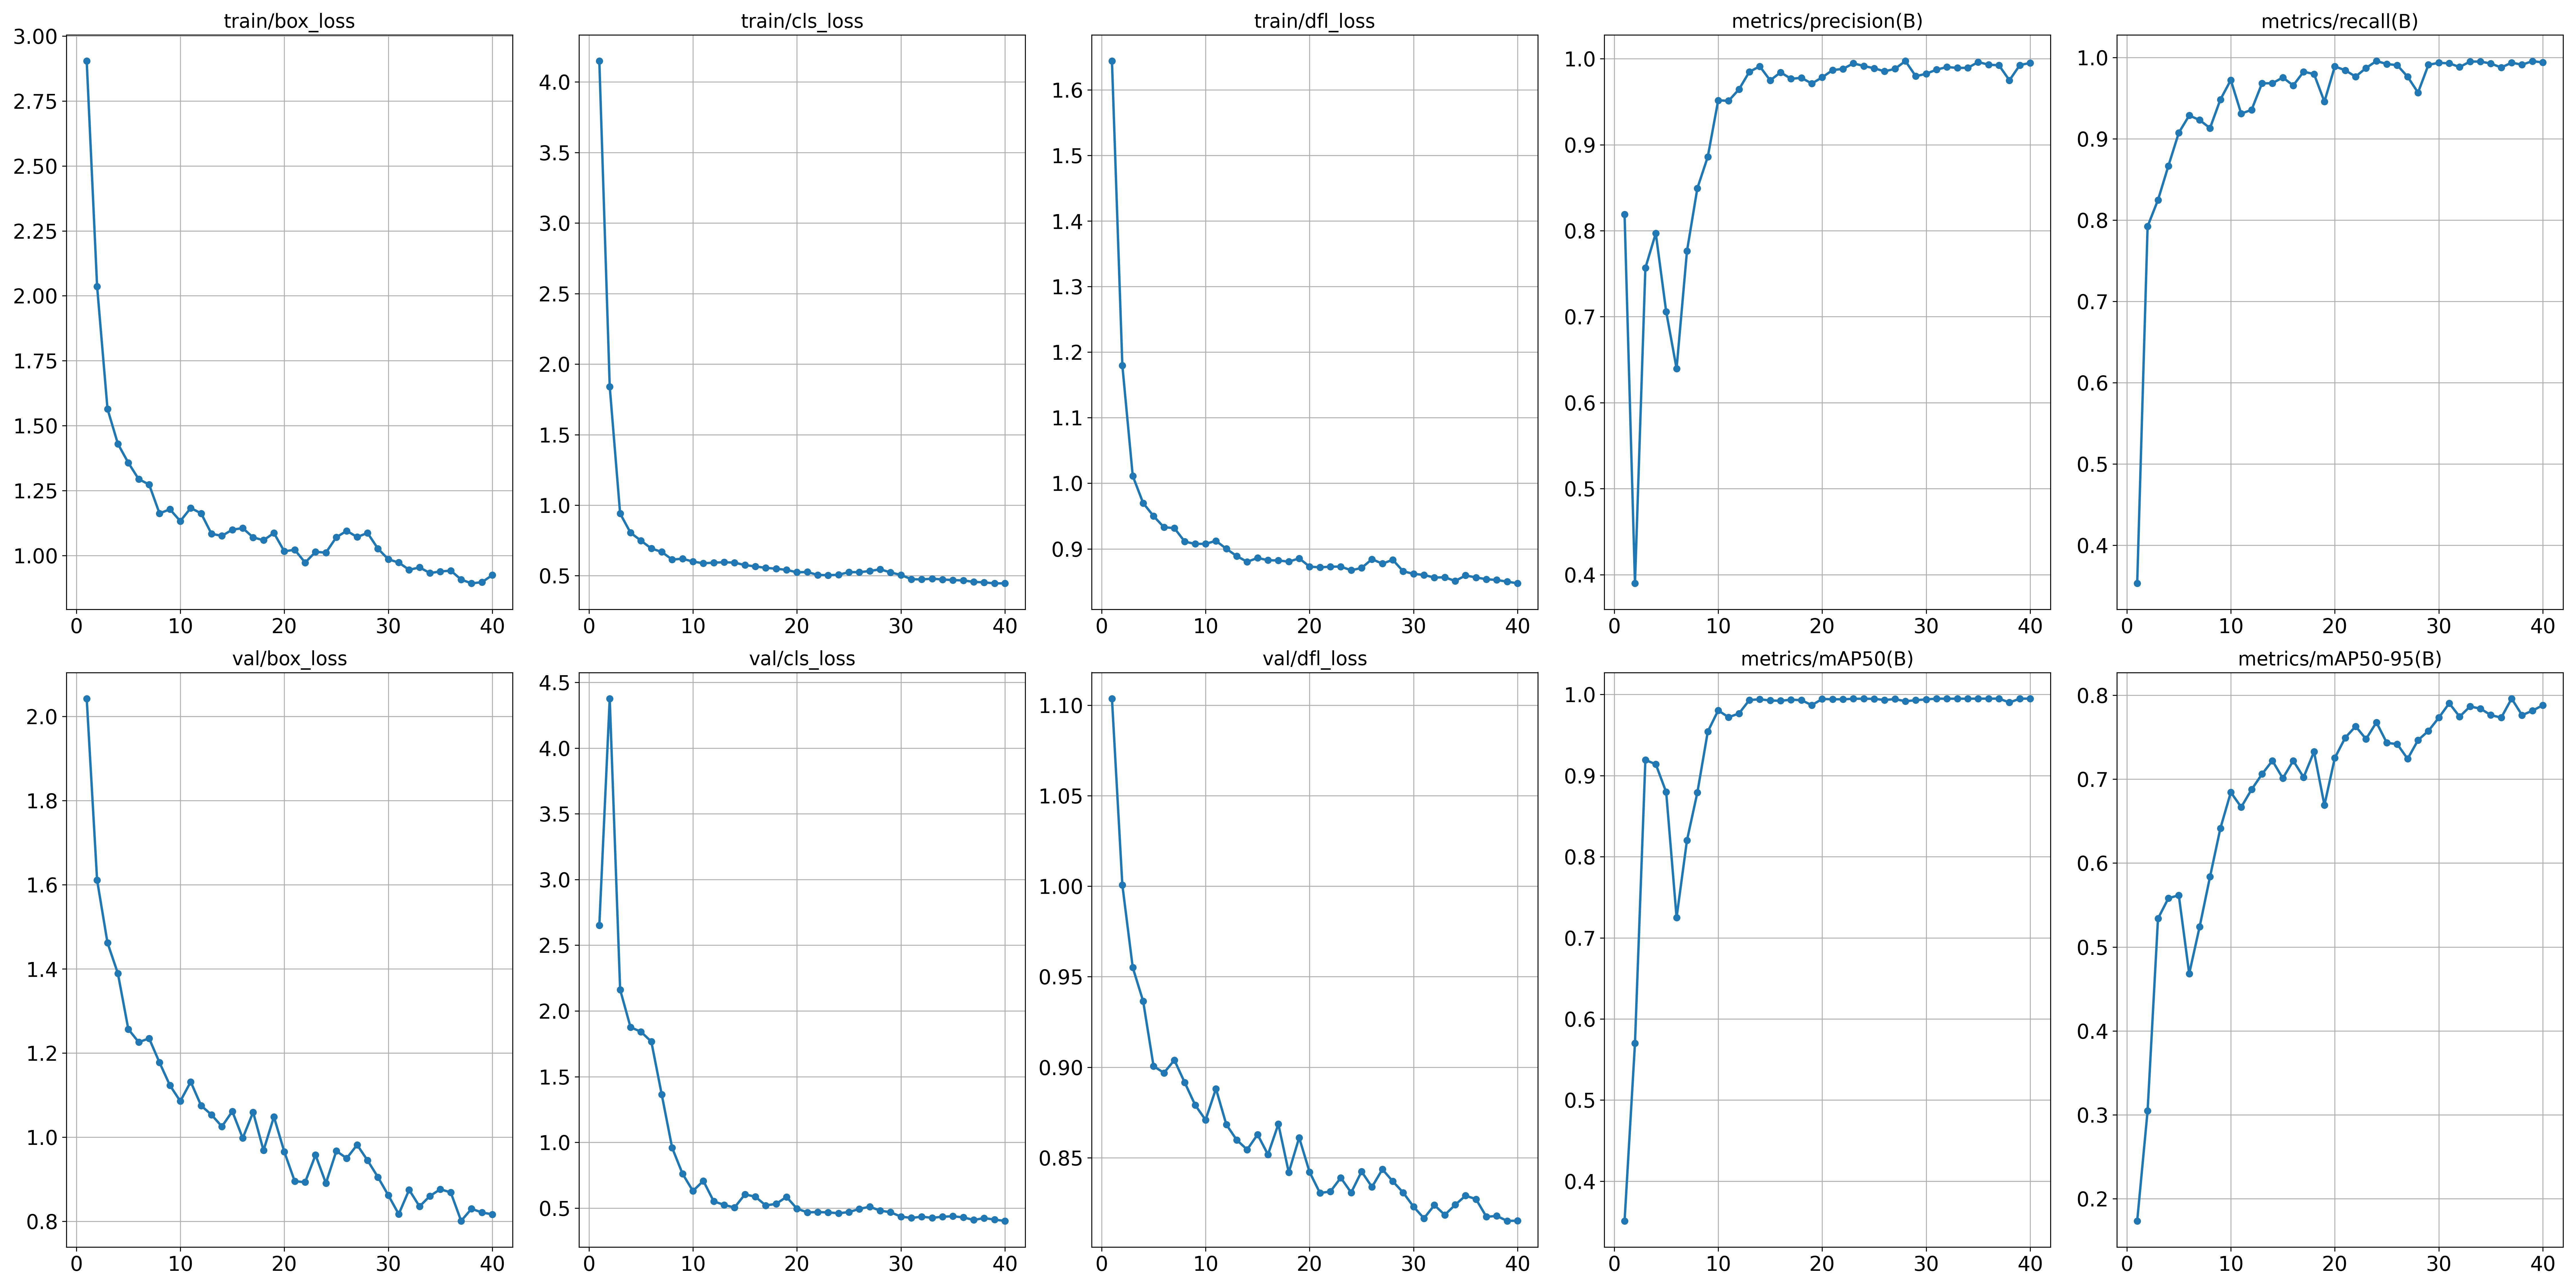
\includegraphics[	
			width=8cm,
			height=7cm,
			keepaspectratio,]{results2.png}
			\\
			(b)
		\end{minipage}
		\newline
		\caption{
			{a) Results.png dosyasının oluşturulması için gereken kod.}
			{b) Results.png dosyasının görüntüsü.}}
	\end{figure}
	\newpage
	\subsection{Gantt Chartların Karşılaştırılması}
	Bu bölümde, ilk projeye başlanıldığında ki gantt chart ile final gantt chartı karşılaştırılmıştır.
	\begin{figure}[!ht]
		\centering
		\includegraphics[
		width=17cm,
		height=10cm,
		keepaspectratio,
		]{eskigantt.png}
		\\
		(a)
	\end{figure}
	\begin{figure}[!ht]
		\centering
		\includegraphics[
		width=17cm,
		height=10cm,
		keepaspectratio,
		]{yenigantt.png}
		\\
		 (b)
		\caption{
			{a) Tasarım raporunun gantt chartı}
			{b) Final raporunun gantt chartı.}}
	\end{figure}
	\\
	Tasarım Gantt şemasına ve final Gantt şemasına bakıldığında, aralarındaki değişiklikler bariz bir şekilde gözükmektedir. Başlangıçta, projenin belirtilen tarihte bitirilmesi planlanmışken, karşılaşılan çeşitli sorunlar ve hatalar nedeniyle proje süresi uzamak zorunda kalmıştır. Bu durum, proje tasarımında her zaman olası hataların ve sorunların çıkabileceği göz önünde bulundurulması ve zaman çizelgesinin buna göre ayarlanması gerektiğini göstermektedir.

	İlk kez bir projeyle uğraşıldığından, projenin nasıl ilerlemesi gerektiği tam olarak anlaşılamamış ve bu da planlama sürecinde eksikliklere yol açmıştır. Haftalık olarak oluşturulan planlamalar, doğru ve yerinde olsaydı, projede daha disiplinli ve net bir ilerleme sağlanabilirdi. Bu sayede projenin takibi ve yönetimi daha kolay ve etkili bir hale gelebilirdi.

	Projeye başlamadan önce, hazırlık aşamaları doğru bir şekilde belirlenmeli ve detaylı bir planlama yapılmalıdır. Başlangıç Gantt şeması, temel yapılandırma ve öğrenme süreçlerine odaklanırken, bu aşamaların titizlikle yürütülmesi gerektiği anlaşılmıştır. Örneğin, "Plaka Tespit Sistemi Yapısının Oluşturulması" ve "Makine Öğrenimine Hazırlık" gibi görevler, projenin temelini oluşturmakta ve başarılı bir ilerleme için kritik öneme sahiptir. Bu aşamalarda yapılan hatalar, projenin ilerleyen safhalarında daha büyük sorunlara yol açabilmektedir.

	Bu deneyimden çıkarılacak önemli bir ders, proje planlamasında esnekliğin ve detaylı zaman yönetiminin önemidir. Proje sürecinde karşılaşılan beklenmedik durumlar için yeterli zaman ve kaynak ayrılmalı, düzenli olarak yapılan değerlendirmelerle planlar güncellenmelidir. Böylece, proje sürecinin daha sağlıklı ve başarılı bir şekilde ilerlemesi sağlanabilir. Ayrıca, ilk kez bir projeyle uğraşan ekipler için detaylı bir rehber ve yol haritası oluşturulması, projenin daha sorunsuz ve verimli bir şekilde tamamlanmasına yardımcı olacaktır. 

	\section{SONUÇ}
	Raporda belirtilen tüm veriler ve analizler sonucunda, geliştirilen akıllı otopark sistemi, hem otopark işletmecilerine hem de kullanıcılara büyük avantajlar sağlamaktadır. Plaka tanıma, araç tespiti ve doluluk belirleme gibi önemli özellikleriyle bu sistem, hızlı giriş/çıkış işlemleri, sorunsuz park etme ve güvenlik takibi gibi konularda önemli iyileştirmeler sunmaktadır. Bu proje, farklı hava koşullarında bile etkin bir şekilde çalışabilen veri setleri kullanılarak geliştirilmiş, derin öğrenme tekniklerinin otopark sistemlerine nasıl entegre edilebileceğini başarılı bir şekilde göstermiştir. Sonuç olarak, bu yenilikçi yaklaşım, şehir içi ulaşımın optimizasyonuna ve kullanıcı deneyiminin iyileştirilmesine önemli katkılar sağlayacaktır.
	
	\newpage
	\bibliographystyle{ieeetr}
	\bibliography{reference.bib}
	\dots{}
\end{document}
